\documentclass[a4paper, 12pt]{article}

%%%%%%%%%%%%%%%%%%% Packages

\usepackage[french, english]{babel}
\usepackage[noheader]{packages/sleek}
\usepackage{packages/sleek-title}
\usepackage{packages/sleek-theorems}

%%%%%%%%%%%%%%%%%%% Titlepage

\logo{./resources/pdf/logo.pdf}
\institute{University of Liège}
\title{Big Data - Review 4}
\subtitle{Renewable Energy Production Forecast}
\author{Yann \textsc{Claes}\\Gaspard \textsc{Lambrechts}\\François \textsc{Rozet}}
%\context{}
\date{\today}

%%%%%%%%%%%%%%%%%%% Bibliography

\addbibresource{./resources/bib/references.bib}

%%%%%%%%%%%%%%%%%%%

\begin{document}
	\maketitle

	\section{Photovoltaic production}

	This section will describe the improvements that were made to both current models and discuss their future use.
	
	\subsection{Panel-wise model}

	As mentioned in the previous review, the model built for the Sart-Tilman is now complete, and we don't plan on improving it even more since it was a startup model and the goal is to predict the energy production at the scale of the city/province of Liège.
	
	For that purpose, we refreshed the latter model to make it more modular in order to be ready (to some extent) to receive as input photovoltaic enumeration data. That is, we moved the Sart-Tilman model onto a file named \texttt{sart-tilman.py} and implemented in the file \texttt{solar.py} a model that should be combined with our photovoltaic panel detector.
	
	To combine our photovoltaic panel detector with our panel-wise model, we plan (hopefully) to use the outputs of the detector. It should yield, at least (for each detected panel/set of panels) :

	\begin{itemize}
	    \item Its corresponding latitude
	    \item Its corresponding longitude
	    \item Its corresponding area
	\end{itemize}

	To get more reliable results, we observed on the Sart-Tilman that computing the incidence angle was quite a big deal, thus we would need to compute that angle. Nevertheless, this angle requires knowledge about the tilt and surface azimuth of the panel. The second one could be easily computed (at first sight); however the tilt of each panel seems quite hard to deduce.
	
	With all these information, we should be able to compute the power output of each PV panel as follows :
	\begin{equation*}
	    P = \eta I A \frac{\cos(\theta)}{\sin(\psi)} 
	\end{equation*}
	where $\eta$ is the efficiency, $I$ is the forecast irradiance, $A$ is the panel area (output of the detector) and $\psi$ is the solar altitude (function of the latitude and longitude of the panel).
	
	One can notice that, in addition to the tilt and surface azimuth, another unknown is the panel efficiency. To deal with all these uncertainties, we could potentially try and use a probabilistic model on top of this physical model (using \texttt{PyStan} for instance), if it seems appropriate.
	
	A sample execution was implemented in \texttt{solar.py}, with user-coded coordinates and parameters, showing the kind of inputs the program expects and plotting the corresponding energy production for the specified forecast period. For now, the irradiance data that is used comes from the CAMS radiation service, which doesn't provide forecast data, but rather historical data (up to two days ago). Later, a forecast API will be used, but we are still looking for a (free) reliable one.
	
	\subsection{Provincial model}

	This model is concerned with the prediction of the energy production at the scale of the province of Liège. As explained during the previous review, it uses radiation data (from the CAMS radiation service, providing global horizontal irradiance data at ground level) in Liège to produce an estimation of the provincial output power as follows :
	\begin{equation*}
	    P = \eta I A
	\end{equation*}
	where $\eta$ corresponds to the efficiency, $I$ the irradiance data and $A$ is a rough measure of the PV area we have in the province of Liège. The latter is the product of the installed power in the province of Liège (\si{\kilo\watt Peak}) and of some measure of average panel area per \si{\kilo\watt Peak} in Belgium (\si{\meter\squared\per\kilo\watt Peak}). Thus, all parameters are, in some sense, arbitrarily fixed in advance, which leads to the example results of Figure \ref{fig:province_example}, for the 21\up{st} of February 2019.
	
	\begin{figure}[H]
	    \centering
	    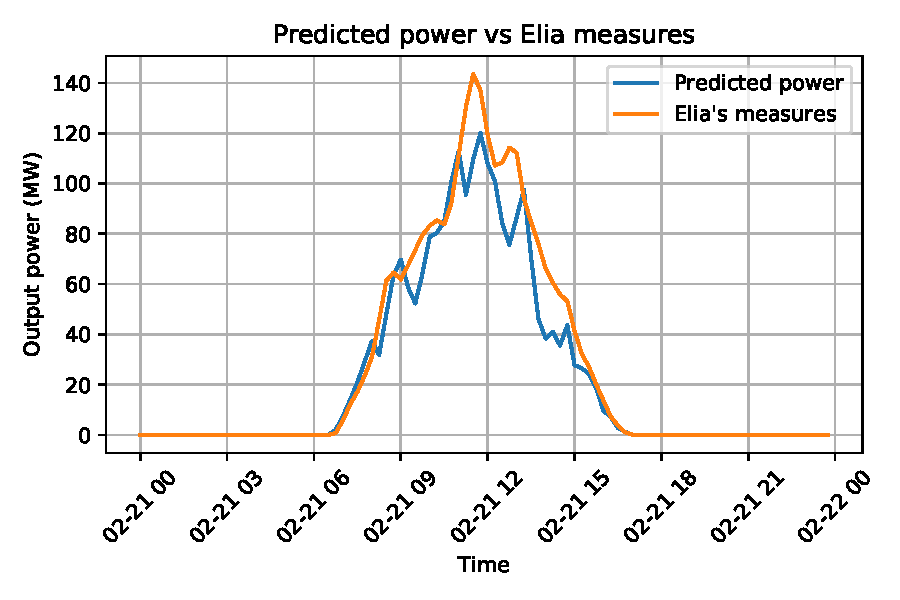
\includegraphics[width=.75\textwidth]{resources/pdf/province_example.pdf}
	    \noskipcaption{Naive physical model example.}
	    \label{fig:province_example}
	\end{figure}
	
	As one can see, the model isn't too bad, but the fact of setting the parameters to some fixed value is too restrictive. For that purpose, we implemented a probabilistic model in PyStan in order to define uncertainties on:

	\begin{itemize}
	    \item $\eta$
	    \item The installed power
	    \item The peak area
	    \item The irradiance
	\end{itemize}

    and, therefore, to define uncertainty on the resulting output model. At the same time, we fit our parameters to Elia's measures (they will in the end be represented by posterior distributions) and we also predict the output power for a given forecast period.
    
    For example, we can fit our parameters on a period ranging from the 15\up{th} of February 2019 to the 23\up{rd} (excluded) and predict for the next day (\emph{i.e.} 23\up{rd} of February).
	
	We can now compare the forecast output power that we would get with our \emph{fixed-parameterized} model with the one we get with PyStan. This comparison can be seen on Figure \ref{fig:comparison_naive_post}.
	
	\begin{figure}[H]
	    \centering
	    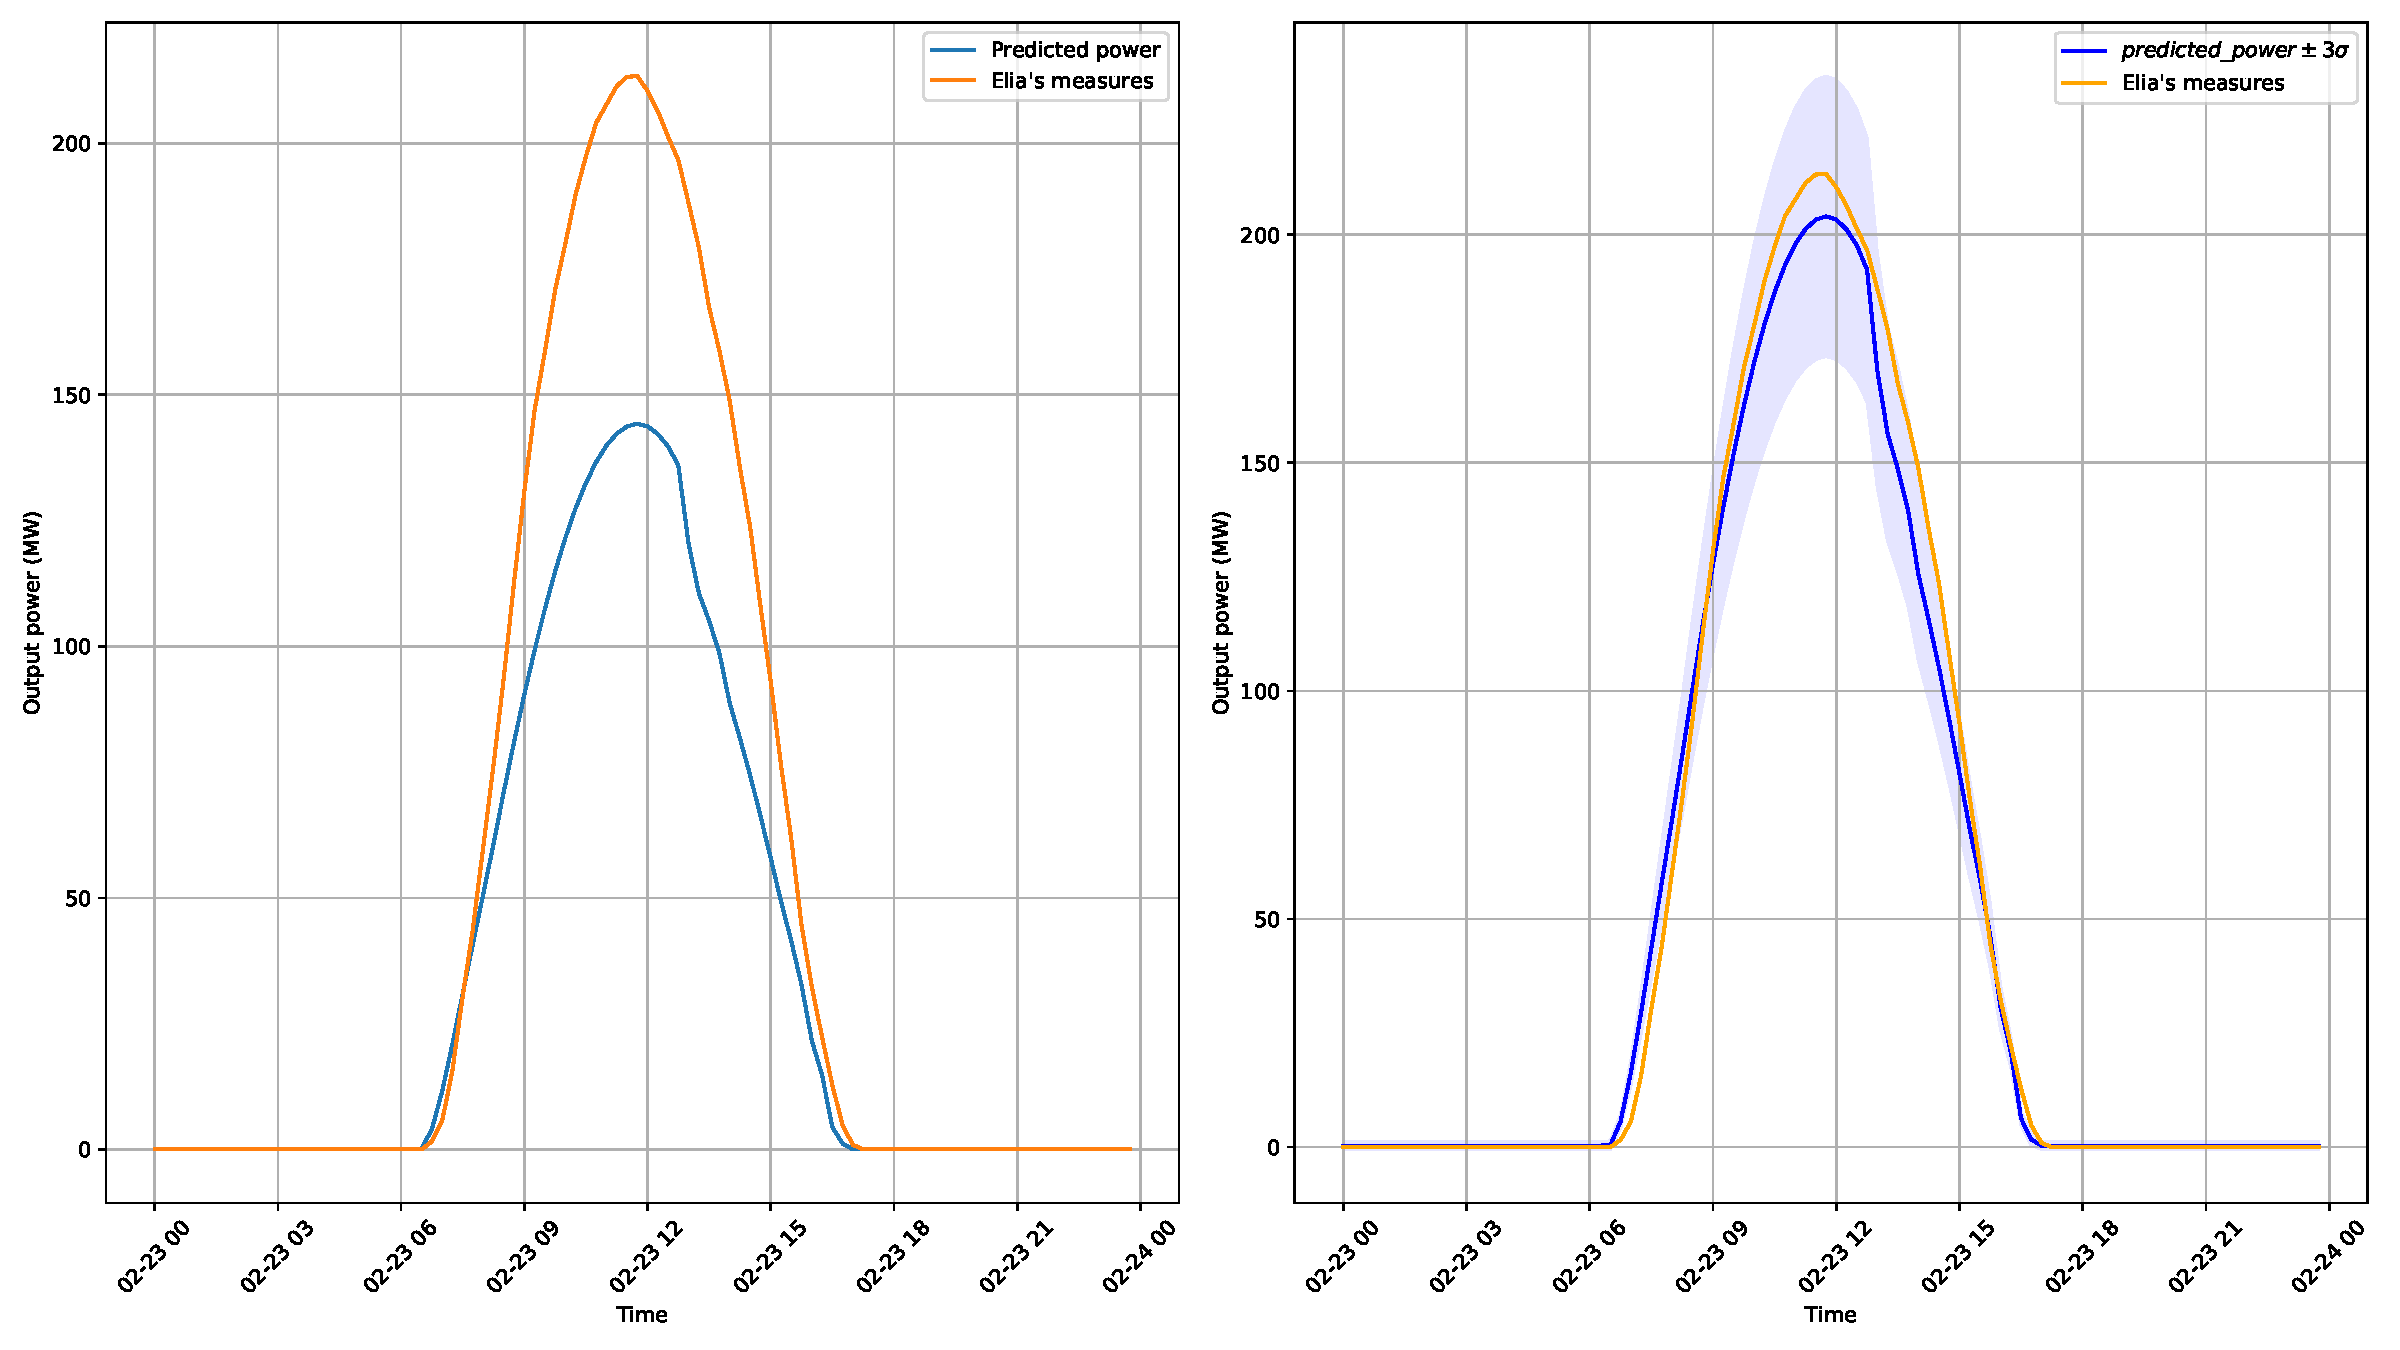
\includegraphics[width=\textwidth]{resources/pdf/comparison_naive_post.pdf}
	    \noskipcaption{Comparison between prior and posterior predictive models.}
	    \label{fig:comparison_naive_post}
	\end{figure}

	We can clearly see that the fitted model performs better at predicting the output power than the naive one. Note that the predictive model is defined as a normal distribution centered around
	$\mu = \eta I A$ with a standard deviation $\sigma = \SI{100}{\kilo\watt}$ (where $\eta$, $I$ and $A$ are sampled by the model\footnote{See \texttt{province.ipynb} for full details.}).  
	
	To get more insight about this, we can compute the mean square error, as well as the root mean square error, which is a nice metric if we want to estimate the standard deviation of our residuals (and therefore, estimate the quality of the prediction) and which is also commonly used for assessing forecasts\cite{bocquet}. To have a more representative metric, we decided to not take into account night observations. We get the results of Table \ref{tab:naive_post} (still for this sample example), using the mean posterior model as reference for our probabilistic model.
	
	\begin{table}[H]
    	\centering
        \begin{tabular}{l|l|l}
                  & MSE      & RMSE   \\ \hline
        Naive     & 2211.522 & 47.027 \\ \hline
        Posterior & 126.439  & 11.244
        \end{tabular}
        \noskipcaption{MSE and RMSE for the naive and posterior models.}
        \label{tab:naive_post}
    \end{table}
	
	Although these results are obviously not representative of all cases we could have (in terms of shape for Elia's measures), the main point is to notice that, by introducing a probabilistic model, we managed to reduce greatly the errors we make on our predictions. By contrast, we can look at the errors Elia makes on their prediction values. This can be seen on Figure \ref{fig:comparison_elia_post}.
	
	\begin{figure}[H]
	    \centering
	    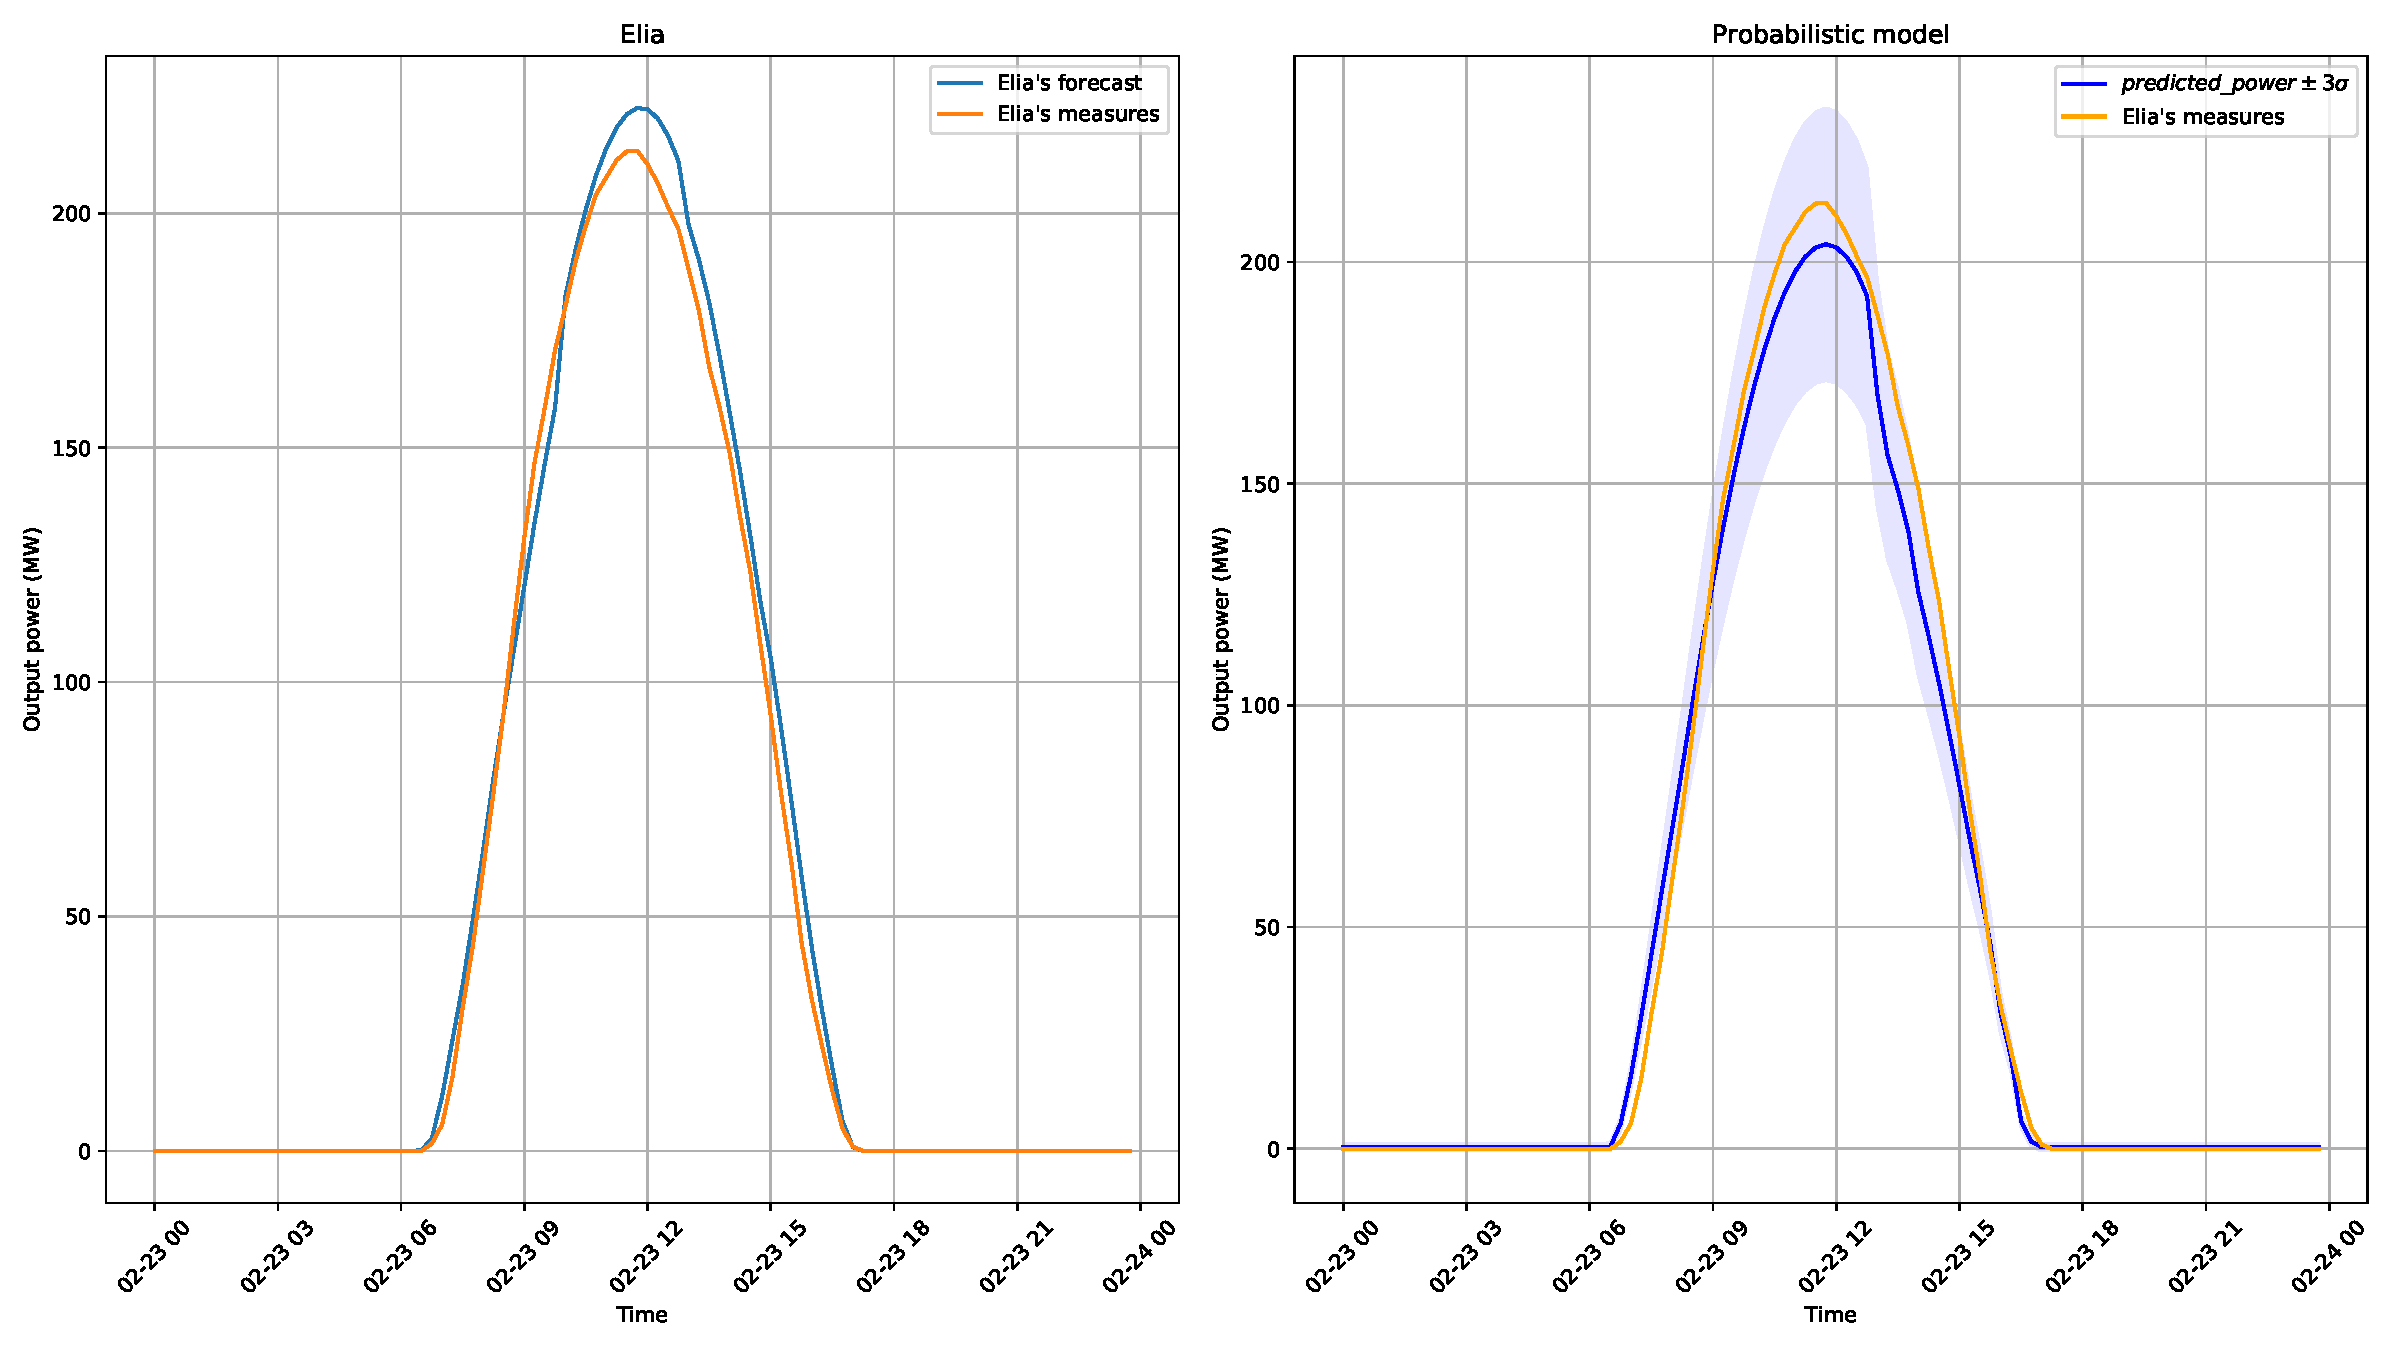
\includegraphics[width=\textwidth]{resources/pdf/comparison_elia_post.pdf}
	    \noskipcaption{Comparison between Elia's forecast and the posterior model.}
	    \label{fig:comparison_elia_post}
	\end{figure}

	As one could expect, it seems that Elia performs slightly better than our probabilistic model. This could be explained by the fact that Elia probably does not (or does not only) rely on a simple physical model as we do. This is also reflected in Table \ref{tab:elia_post}.
	
	\begin{table}[H]
    	\centering
        \begin{tabular}{l|l|l}
                  & MSE      & RMSE   \\ \hline
        Elia      & 84.988 & 9.219    \\ \hline
        Posterior & 126.439  & 11.244
        \end{tabular}
        \noskipcaption{MSE and RMSE for Elia's predictions and the posterior model.}
        \label{tab:elia_post}
    \end{table}
    
    Nevertheless, we shouldn't draw hasty conclusions. Indeed, doing the same experiment on the next month had the effect of pushing up the parameters too much (w.r.t. the naive predictions), leading to a higher overestimation of the power forecast, as can be seen on Figure \ref{fig:bad_naive_post}, while Elia's forecast is still on point, as can be observed on Figure \ref{fig:bad_elia_post}.
    
    \begin{figure}[H]
        \centering
        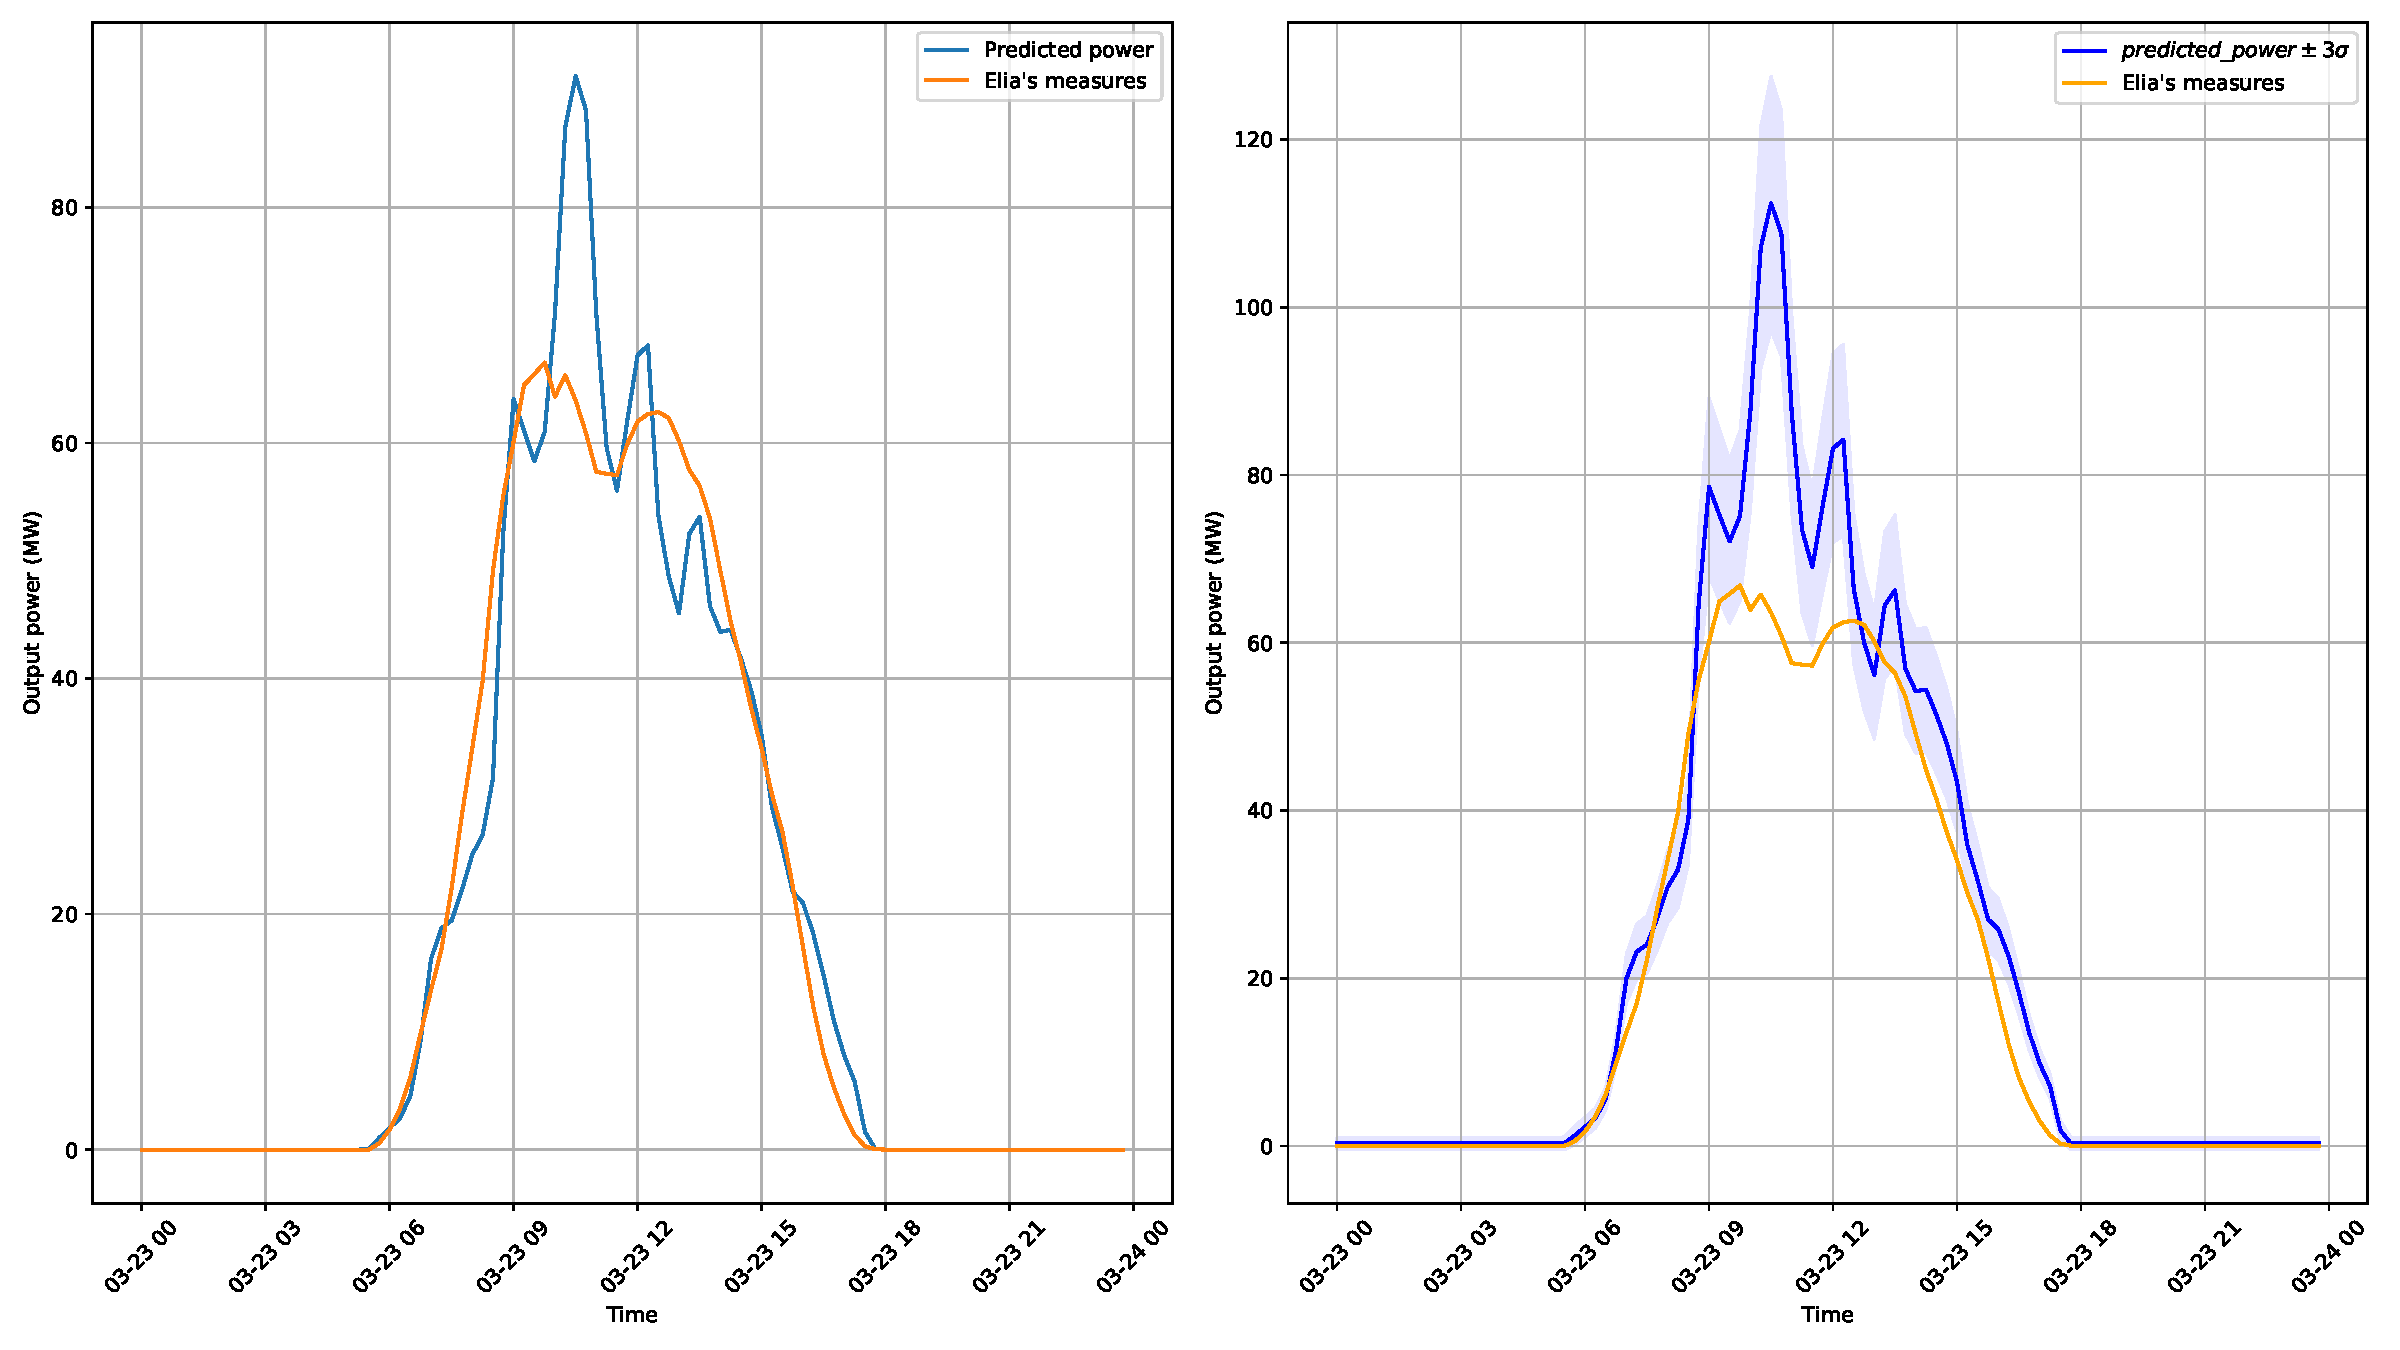
\includegraphics[width=\textwidth]{resources/pdf/bad_naive_post.pdf}
        \noskipcaption{Same example for March 2019 (naive vs posterior model).}
        \label{fig:bad_naive_post}
    \end{figure}
    
    \begin{figure}[H]
        \centering
        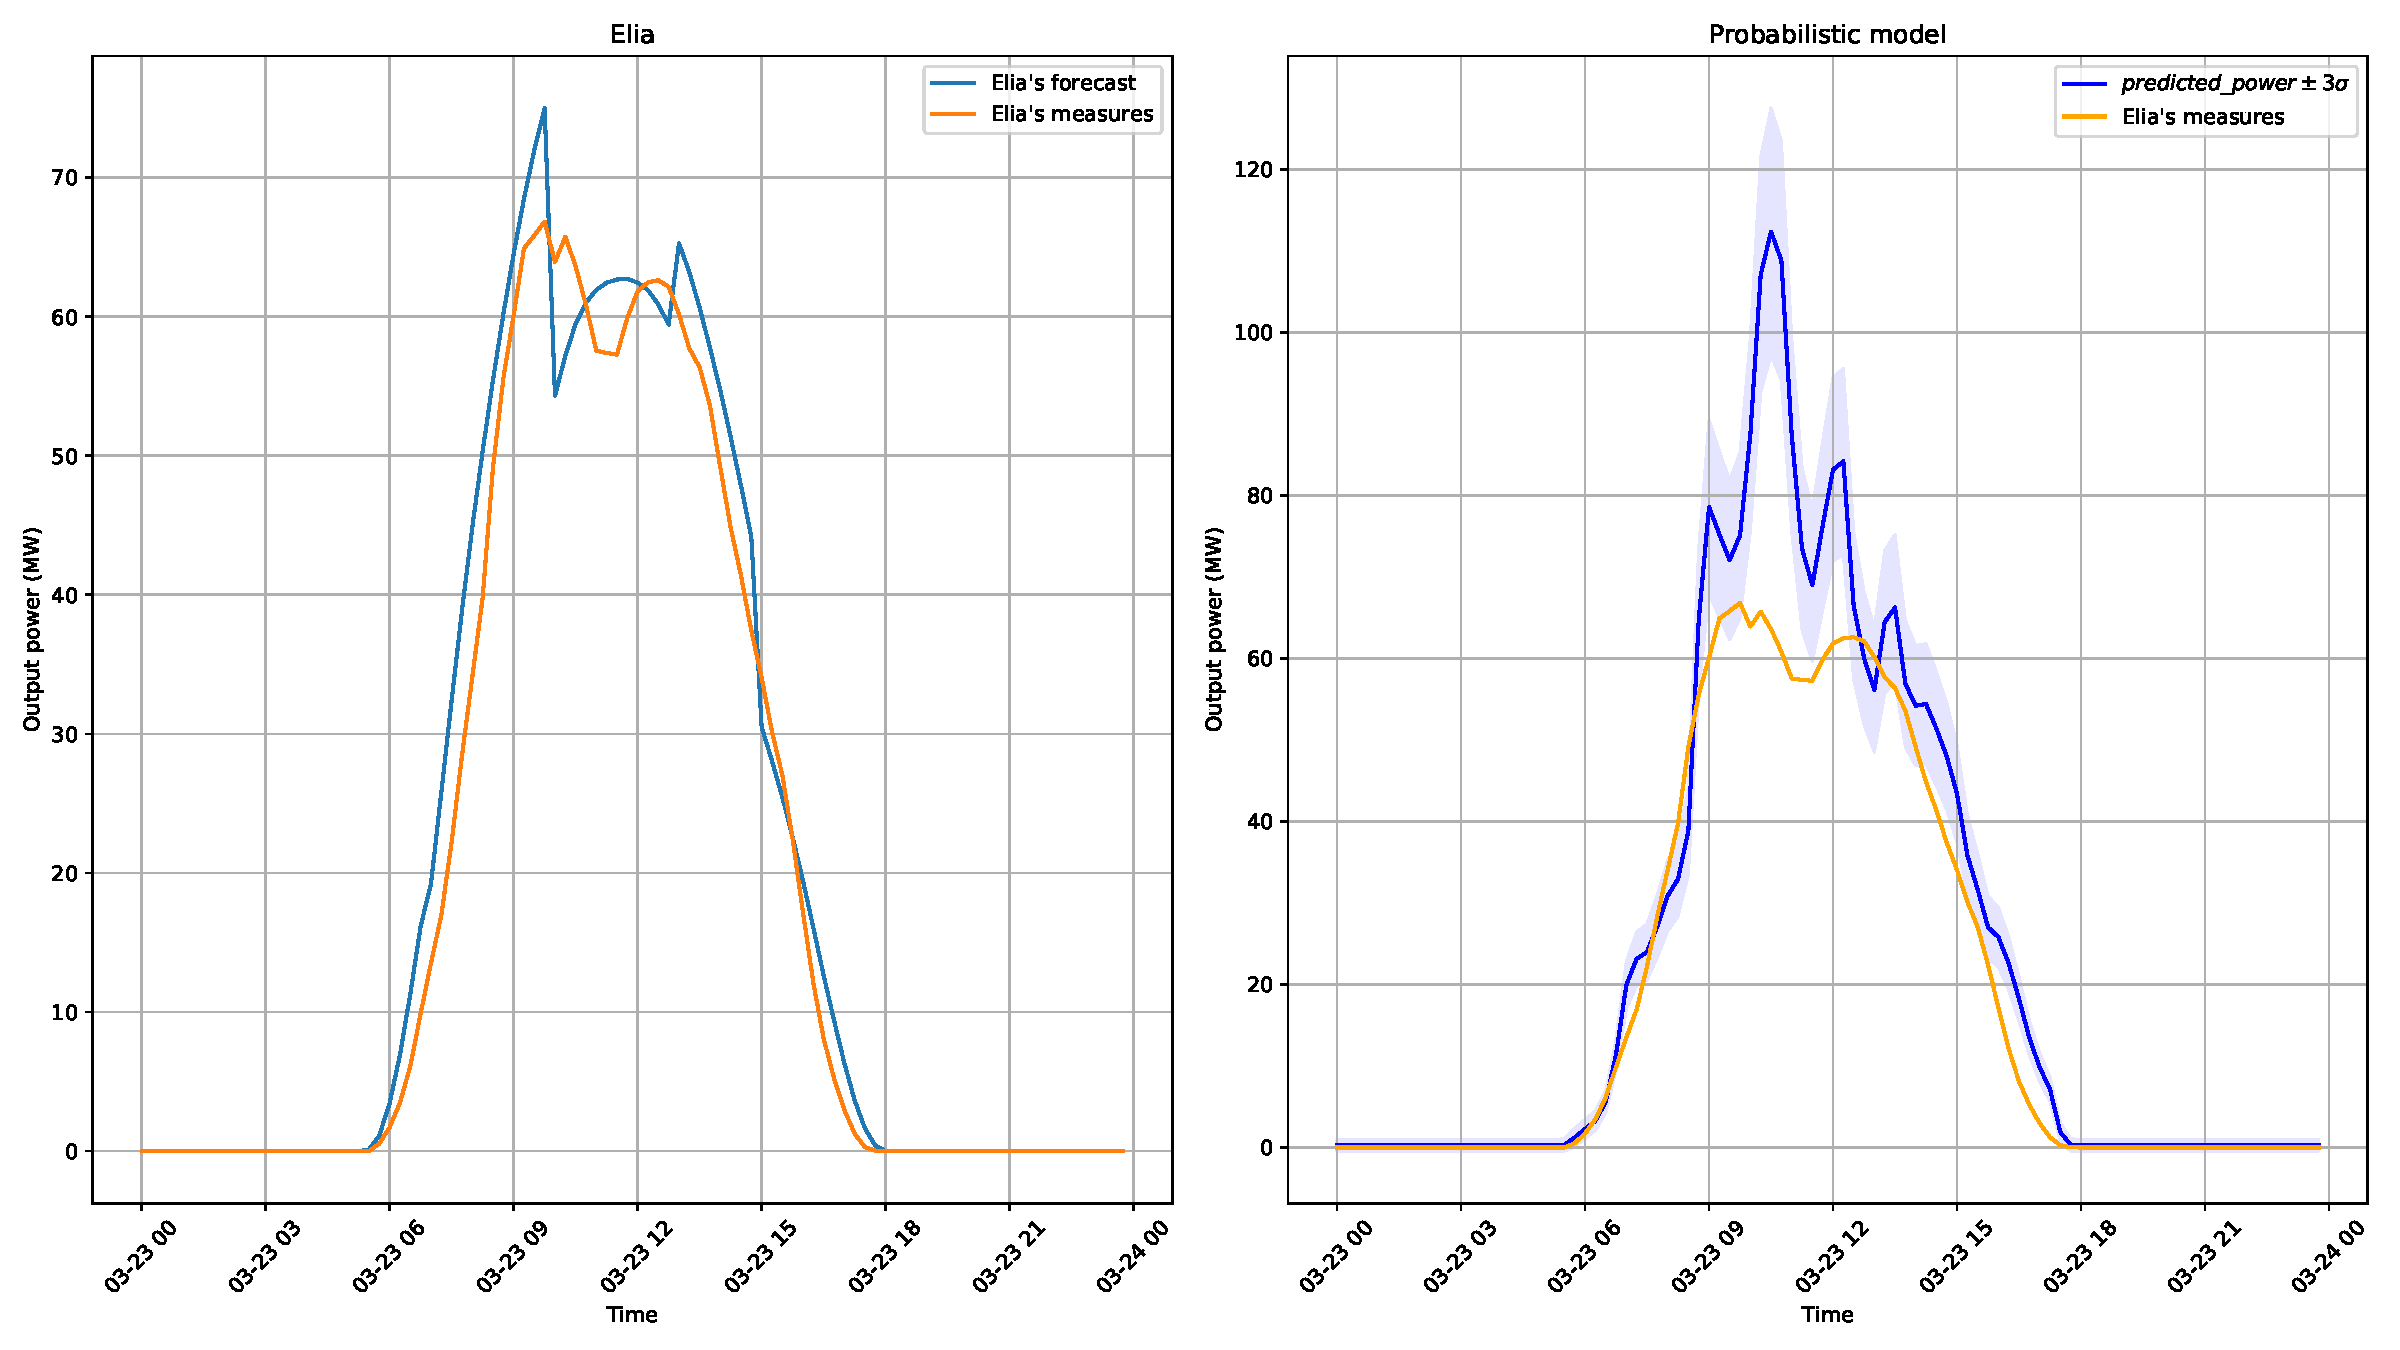
\includegraphics[width=\textwidth]{resources/pdf/bad_elia_post.pdf}
        \noskipcaption{Same example for March 2019 (Elia vs posterior model).}
        \label{fig:bad_elia_post}
    \end{figure}
    
	\subsection{Irradiance data}

	For now, no free and reliable forecast API have been found to retrieve irradiance data in Liège. Indeed, the only one we have so far is Climacell, but as was already said, the measures they provide seem to be quite underestimating the true irradiance that is observed. We thus only use the data coming from the CAMS radiation service, that only provides historical data.
	
	A potential alternative could be HelioClim-3 \cite{helioclim}, but no free automatic access can be obtained, and once again, there seems to be unreliable measurements: they tend to highly overestimate the true irradiance (since they are expressed in \si{\watt\hour\per\meter\squared}, a conversion is needed to get \si{\watt\per\meter\squared}).

	\subsection{Next objectives}

	In addition to trying to find a reliable irradiance forecast API, it would be nice to find an API that combines both historical data as well as forecast data. Indeed, since the irradiance plays a crucial role in the produced power in our models, fitting parameters on some irradiance data coming from source 1 and predicting the output power using irradiance data coming from source 2 will definitely be more biased than if we use irradiance data coming from the same source.
	
	What remains to be done to complete the analysis of such a posterior model is to compare the latter with simple baseline models (moving average of the output power over the last D days, etc.) as well as to evaluate the posterior model over a representative period (and eventually compare with what Elia obtains over such a period).

    \newpage
    
    \section{Photovoltaic panels enumeration}
    
    As a quick reminder, we have already obtained a suitable dataset for training : a large collection of \emph{publicly available} [\href{https://energy.duke.edu/content/distributed-solar-pv-array-location-and-extent-data-set-remote-sensing-object-identification}{link}] high resolution aerial imagery, with over \num{19000} human annotated PV panels locations.
    
    Our goal is now to design and train a neural network able to \emph{detect} photovoltaic (or solar) panels in satellite images, hence the name \emph{Automatic Detection Of Photovoltaic Panels Through Remote Sensing} or ADOPPTRS\footnote{This part of the project is conducted in parallel with our project of \emph{Deep Learning}. Therefore, we have created another GitHub repository especially for this purpose : \texttt{\href{https://github.com/francois-rozet/adopptrs}{https://github.com/francois-rozet/adopptrs}}.}.
    
    \begin{note}
        What we discovered recently is that this collection was released with the paper \og{}Automatic Detection of Solar Photovoltaic Arrays in High Resolution Aerial Imagery\fg{} \cite{malof2016automatic} from Duke University from which our sub-project name is inspired. Interestingly, this paper didn't use neural networks for detection but Random Forests instead.
    \end{note}
    
    \subsection{DeepSolar}
    
    The first model we looked after was the one used and designed for the DeepSolar \cite{yu2018deepsolar} project conducted at Stanford University as it is one of the most reviewed. DeepSolar's goal is very similar to ours, \emph{i.e.} detecting all PV panels in the United States using satellite imagery. However, the model used by DeepSolar is fairly complicated. It incorporates both image classification (Google Inception V3 \cite{szegedy2016rethinking}) and semantic segmentation in a single convolutional neural network.
    
    \begin{figure}[h]
        \centering
        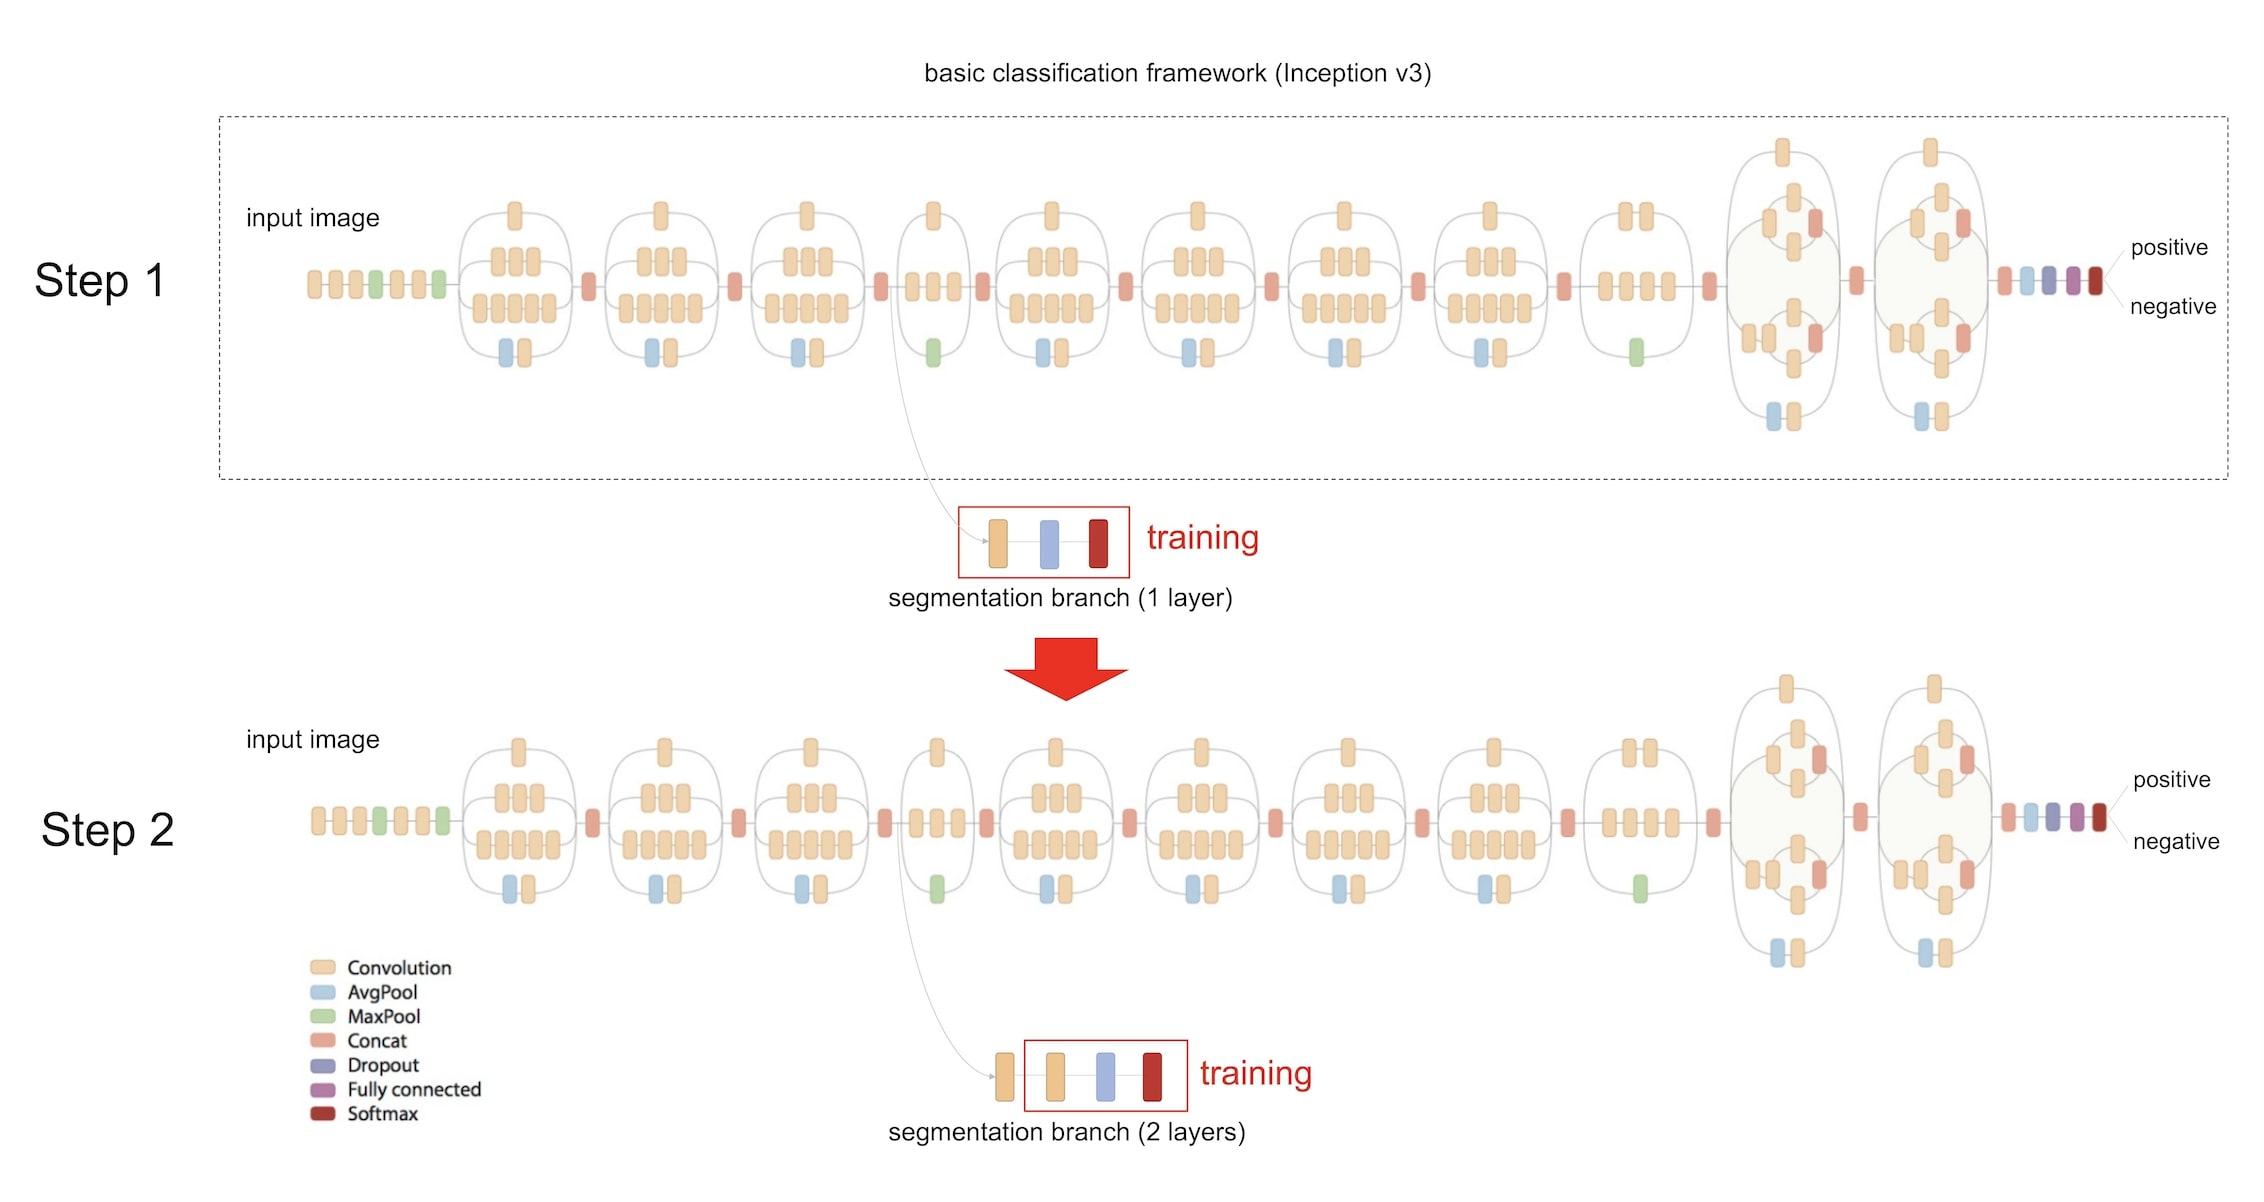
\includegraphics[width=\textwidth]{resources/jpg/cnn_arch.jpg}
        \caption{DeepSolar's network representation. \cite{yu2018deepsolar}}
    \end{figure}
    
    The classification branch is used to localize the solar panels and the segmentation one to estimate their sizes. Only if an image is classified as \emph{positive} (containing a PV panel), the segmentation branch is executed. The advantage of this method is that the segmentation does \emph{not} need another forward pass. Unfortunately, we believe that reproducing such network is not within our capabilities, at least for now.
    
    Furthermore, the reason why DeepSolar was first built as a classification network was because the researcher(s) didn't have \emph{segmentation} masks as training set. In fact they only had images with \emph{labels} indicating the presence or absence of panels. Therefore they had to solve a problem of \emph{semi-supervised} segmentation.
    
    Conversely, we have segmentation masks (cf. previous review) and therefore we can train directly a segmentation model.
    
    \subsection{U-Net}
    
    One of the most famous segmentation model is U-Net \cite{ronneberger2015u}. Initially designed for biomedical image segmentation, it actually works very well for a lot of applications.
    
    \begin{figure}[H]
        \centering
        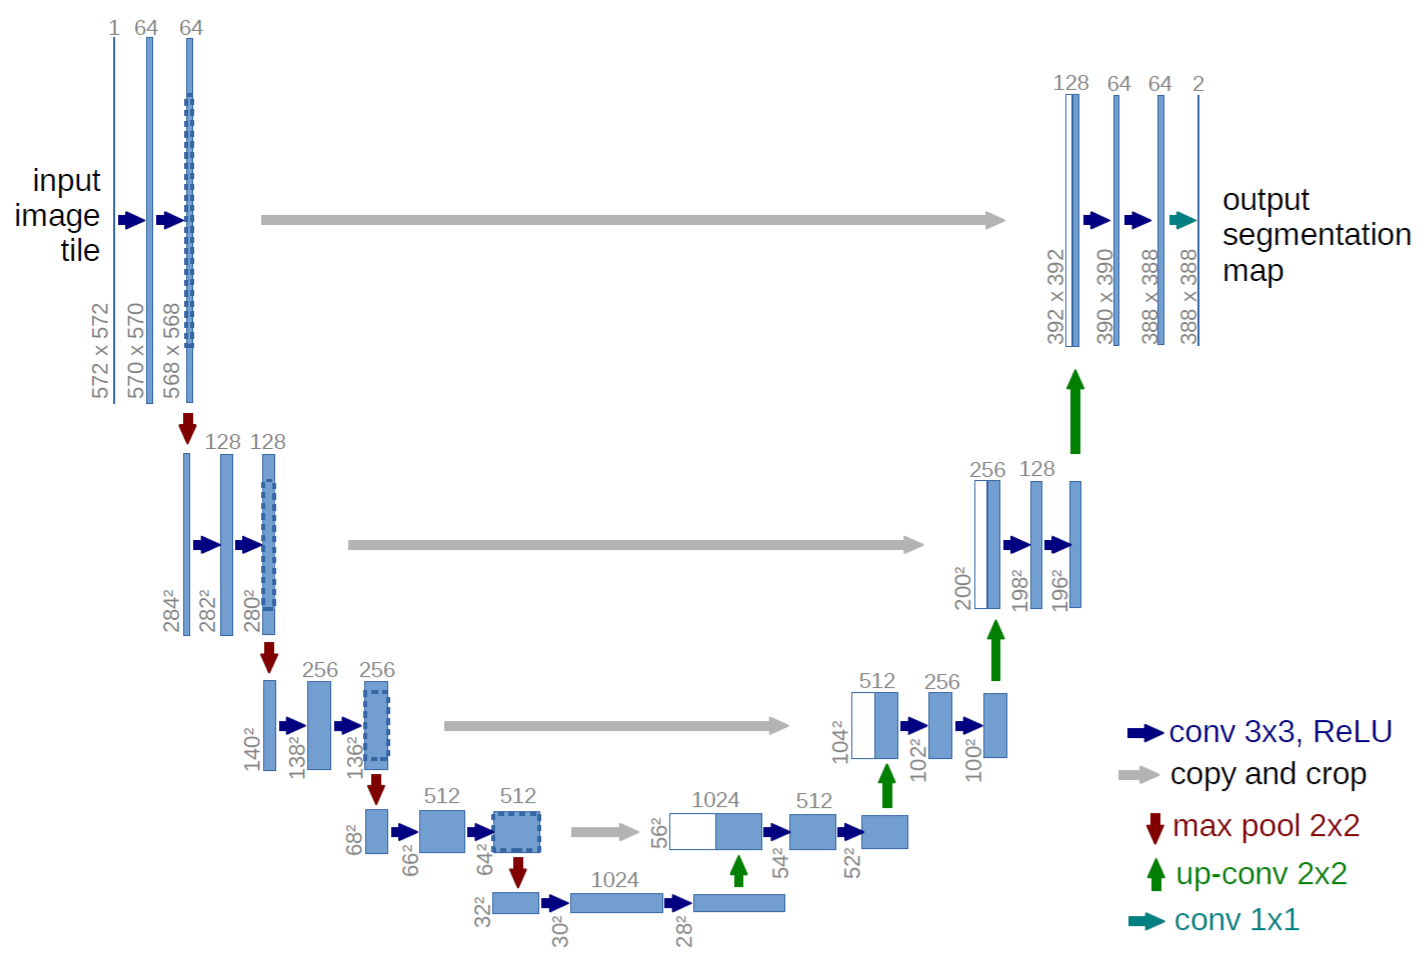
\includegraphics[width=0.9\textwidth]{resources/png/unet.png}
        \caption{U-net architecture. \cite{ronneberger2015u}}
    \end{figure}
    
    We have implemented and trained this model using \texttt{PyTorch}. We first tried with a shortened version of U-Net but it didn't worked very well. We are now using the full architecture.
    
    \subsection{Training}
    
    We divided our dataset in 3 subsets : a training set (\SI{75}{\percent}), a validation set (\SI{12.5}{\percent}) and a testing set (\SI{12.5}{\percent}). The first one will be used for training our models, the second one for selecting the best one (and train it again) and the third one will be used to evaluate our final model (at the very end of our journey).
    
    \subsubsection{Loss function}
    
    One of the most used loss function for segmentation (and classification) is the \emph{cross entropy loss} function.
    \begin{equation*}
        CrossEntropy(\hat{\bm{y}}, \bm{y}) = - \sum_{c=1}^C y_c \log \hat{y}_c
    \end{equation*}
    where $\hat{\bm{y}} \in \sbk{0, 1}^C$ is the model probability distribution prediction among the $C$ classes and $y \in \cbk{0, 1}^C$ is the ground truth. For a binary classification problem as we face, this reduces to
    \begin{equation*}
        BinaryCrossEntropy(\hat{y}, y) = - y \log \hat{y} - (1 - y) \log (1 - \hat{y})
    \end{equation*}
    We tried using this function (implemented in \texttt{PyTorch} as \texttt{BCELoss}) but the results were quite poor. Indeed, most of our predictions were simply pitch black. We think this is due to the huge class imbalance\footnote{We haven't tried class weighting yet.} in the dataset.
    
    We therefore searched for a \og{}loss function for imbalanced segmentation\fg{} and a lot of forums and websites mentioned the \emph{dice coefficient} and \emph{intersection over union}. Conversely to the cross entropy, these metrics are not applied pixel-wise but image-wise (or batch-wise).
    \begin{align*}
        IoU(A, B) & = \frac{\abs{A \cap B}}{\abs{A \cup B}} & Dice(A, B) & = \frac{2 \abs{A \cap B}}{\abs{A} + \abs{B}}
    \end{align*}
    
    \begin{figure}[H]
        \centering
        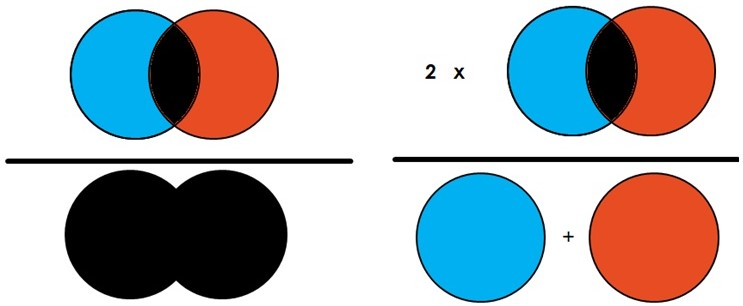
\includegraphics[width=0.9\textwidth]{resources/jpg/iou_dice.jpg}
        \noskipcaption{Illustration of Intersection over Union (left) and Dice Coefficient (right). \cite{towardsdatascience}}
    \end{figure}
    
    Both metrics are very similar but the Dice Coefficient is actually a little bit easier to implement which is why we chose to continue with it.
    
    \begin{note}
        To transform these metrics into loss function we have to consider $1 - Dice$ and $1 - IoU$.
    \end{note}
    
    \subsection{Data augmentation}

    As we have mentioned in the previous review, we wished to increase the size of our dataset trough data augmentation. Our approach is to randomly apply some transformation(s) to the training set \emph{while training}. Therefore, at each epoch, the training set is slightly different and becomes much harder to overfit on.
    
    The implemented transformations are :
    
    \begin{itemize}[noitemsep]
        \item Rotations : \SI{90}{\degree}, \SI{180}{\degree}, \SI{270}{\degree} 
        \item Flipping horizontally or vertically
        \item Brightness alteration
        \item Saturation alteration
        \item Contrast alteration
    \end{itemize}
    
    \begin{figure}[H]
        \centering
        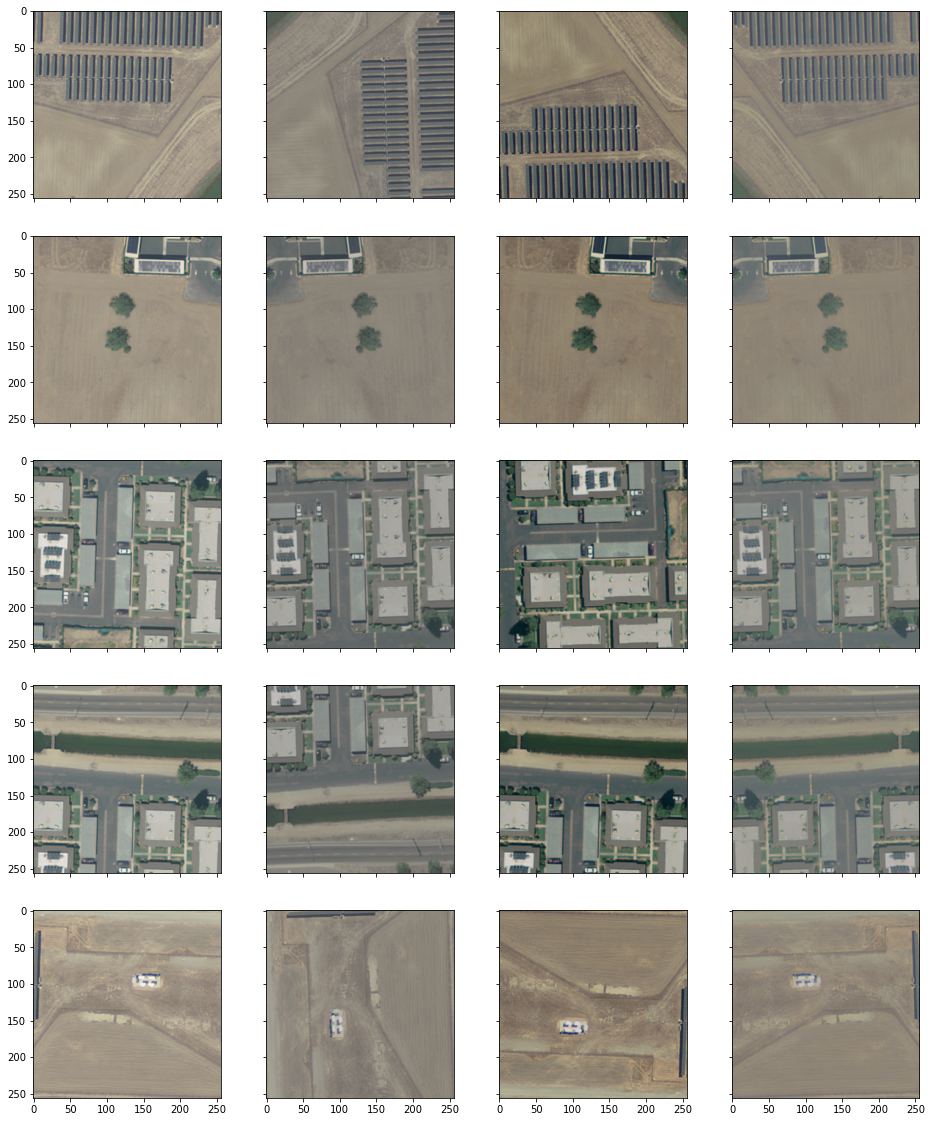
\includegraphics[width=\textwidth]{resources/png/augmentation.png}
        \noskipcaption{Example of some image transformations. The first column is the original.}
    \end{figure}
    
    \subsection{Results}
    
    For the moment, our best model (obtained after 32 epochs in 16 hours\footnote{We actually did way more training phases than this, but we stumbled upon quite a few problems with the GPU clusters.}) achieves an average Dice Loss of \SI{26.5}{\percent} on the validation set (and \SI{16.91}{\percent} on the training set). Pay attention that it is \emph{not} a measure of accuracy ! What should be more informative is the \emph{confusion matrix} :
    
    \begin{table}[H]
        \centering
        \begin{tabular}{cc|cc}
            && \multicolumn{2}{c}{Truth} \\
            && 0 & 1 \\ \hline
            \multirow{2}{*}{Prediction} & 0 & \num{3.236e5} & \num{1.054e3} \\
            & 1 & \num{3.096e2} & \num{2.690e3} \\
        \end{tabular}
        \noskipcaption{Average confusion matrix on the validation set.}
        \label{tab:confusion_matrix}
    \end{table}
    
    As one can see in Table \ref{tab:confusion_matrix}, the majority of our predictions are (rightfully) negative, which emphasises the class imbalance we talked earlier. As a consequence our model reaches an (irrelevant) accuracy of \SI{99.58}{\percent}. Instead, we should consider the \emph{specificity}/\emph{precision} and \emph{sensitivity}/\emph{recall} metrics :
    \begin{align*}
        precision & = \frac{TP}{TP + FP} = \SI{89.69}{\percent} \\
        recall & = \frac{TP}{TP + FN} = \SI{71.92}{\percent}
    \end{align*}
    This precision score means that our model rarely classifies something else as a photovoltaic panel but this recall score means that it often fails to recognize a photovoltaic panel. Yet for a first model this isn't terrible at all !
    
    Some evaluation samples are provided in the appendix.
    
    \subsection{Next objectives}
    
    Even though our first model isn't that bad, we still want to improve it and to try a few other models before applying it to our initial problem.
    
    Also, at each epoch, we evaluated our model on the validation set and saved a few statistical measures about the losses. We could try to analyse convergence through these measures.
    
    Finally, there is still to do a few post-processing to convert the obtained predictions into photovoltaic panel locations.
    
    \newpage
    
    \section{Wind production}

    \subsection{Classification of wind forecasting problems}
    
    \begin{itemize}
        \item Very-short-term or immediate-short-term (a few hour ahead)
        \item Short-term (few hours to several days)
        \item Long-term (multiple days ahead)
    \end{itemize}
    
    \subsection{Classical approaches in Wind Power Prediction}
    
    \label{subsec:classification}
    
    From \emph{Sweeny et. al, 2019} \cite{sweeney2019future} and \emph{Messner et. al, 2020} \cite{messner2020windpower}, we have identified the following approaches for wind power forecasting.

    \begin{enumerate}[label=\arabic*]
        \item \textbf{Physical modeling}: based on Numerical Weather Prediction (NWP), the model aim at outputting the power produced by one power plant using the power plant characteristics (wind turbine power curves, surface roughness and obstacles, terrain wake, hub heights, and even the wind farms wake effect on themselves is taken into account in recent works). These approaches are said to be very computationally expensive, and quite hard to apply on very large scale situation as in our case where we have 64 power plants. However, what we showed in review 2 corresponds to the strategy for physical modelling described in the second paper, with a simpler model.
        \item \textbf{Statistical modeling}
    
        \begin{enumerate}[label=\alph*]
            \item On the very short term: \emph{time series based forecasting}: the NWP data is not used, only the power time series is used to make the prediction. This approach is said to be hard to beat on 4 to 6 hours ahead predictions (very short term).
            \item On the longer term: \emph{post processing of NPW}: the temporal aspect is not considered. The power predictions are based on NWP. Roughly, this approach aim at mimicking the physical model when some information are missing such as the surface roughness and terrain wake effect for each power plant. 
        \end{enumerate}
        \item \textbf{Hybrid method}: uses \emph{post processing of NPW} \textbf{and} \emph{of physical modeling}.
    \end{enumerate}
    
    \emph{For now}, the most promising and adapted approach seems too be the
    \emph{post processing of NPW}, since:
    \begin{itemize}
        \item Our physical model was not good (but could be improved) and we have a big number of wind farms,
        \item We have a good amount of data,
        \item We address the one-day ahead forecasting task,
        \item The results of the simple statistical model of review 3 were promising.
    \end{itemize}
    
    However, the possible improvements on the physical model are considered below, as a hybrid method could perform even better than the statistical modeling.

    \subsection{Physical model}
    
    The physical model that we built for review 2 was constituted of a power curve for each wind turbine. It took as input the wind at each power plant location.
    
    This model could be refined by using the \emph{log wind profile} (semi-empirical relationship) to model the wind at hub height : $$u(z_2) = u(z_1) \frac{\ln(z_2/z_0)}{\ln(z_1/z_0)}$$ where $z_2$ is the height of interest (hub height), $z_1$ is the height at which the wind speed is measured (typically \SI{10}{\meter\per{\second}}), and $z_0$ is the roughness length that measures the roughness of a surface on the wind flow. This value ranges between \num{0.005} and \num{0.1} for onshore wind farm terrains. This parameter would have to be estimated.
    
    It could also be refined by taking into account the wind direction and model the self wake effect due to alignment of wind and wind turbines (the exact location of each wind turbine in Wallonia is known). This would also imply several unknown parameters to estimate.

    \subsection{Statistical model - Weather to Power}
    
    We chose to name the statistical model a \emph{weather to power} model (case 2.b in the classification of section \ref{subsec:classification}) in order to distinguish from the time series modeling.
    
    The statistical model built at the last review was a \emph{wind to power} model where the forecast of wind was considered at a single location. This time, we have built a new training set that is constituted of the following inputs (NPW measured at 15 different locations) :
    
    \resizebox{\textwidth}{!}{
        \begin{tabular}{|c|c|c|c|c|c|c|}
            \hline
            \texttt{windSpeed} & \texttt{windGust} & \texttt{windBearing} & \texttt{temperature} & \texttt{humidity} & \texttt{pressure} & \texttt{airDensity} \\ \hline
            \SI{}{\meter\per{\second}} & \SI{}{\meter\per{\second}} &\SI{}{\meter\per{\second}} & \SI{}{\kelvin} & - & \SI{}{\pascal} & \SI{}{\kilogram\per{\meter\cubed}} \\ \hline
        \end{tabular}
    }
    
    This columns are thus repeated 15 times (one time at each location where the weather forecasts are made), they are thus 105 in total. The forecast locations have been chosen by hand, looking at the map of all wind turbines in Wallonia. The limitation of 15 locations is due to the fact that we use a free weather API. But later, we will certainly retrieve these 7 weather data-points at each power plant.
    
    On the figure \ref{fig:power_plants}, we can see the locations of each power plant and in red the location of the weather measures.

    \begin{figure}[h!]
        \centering
        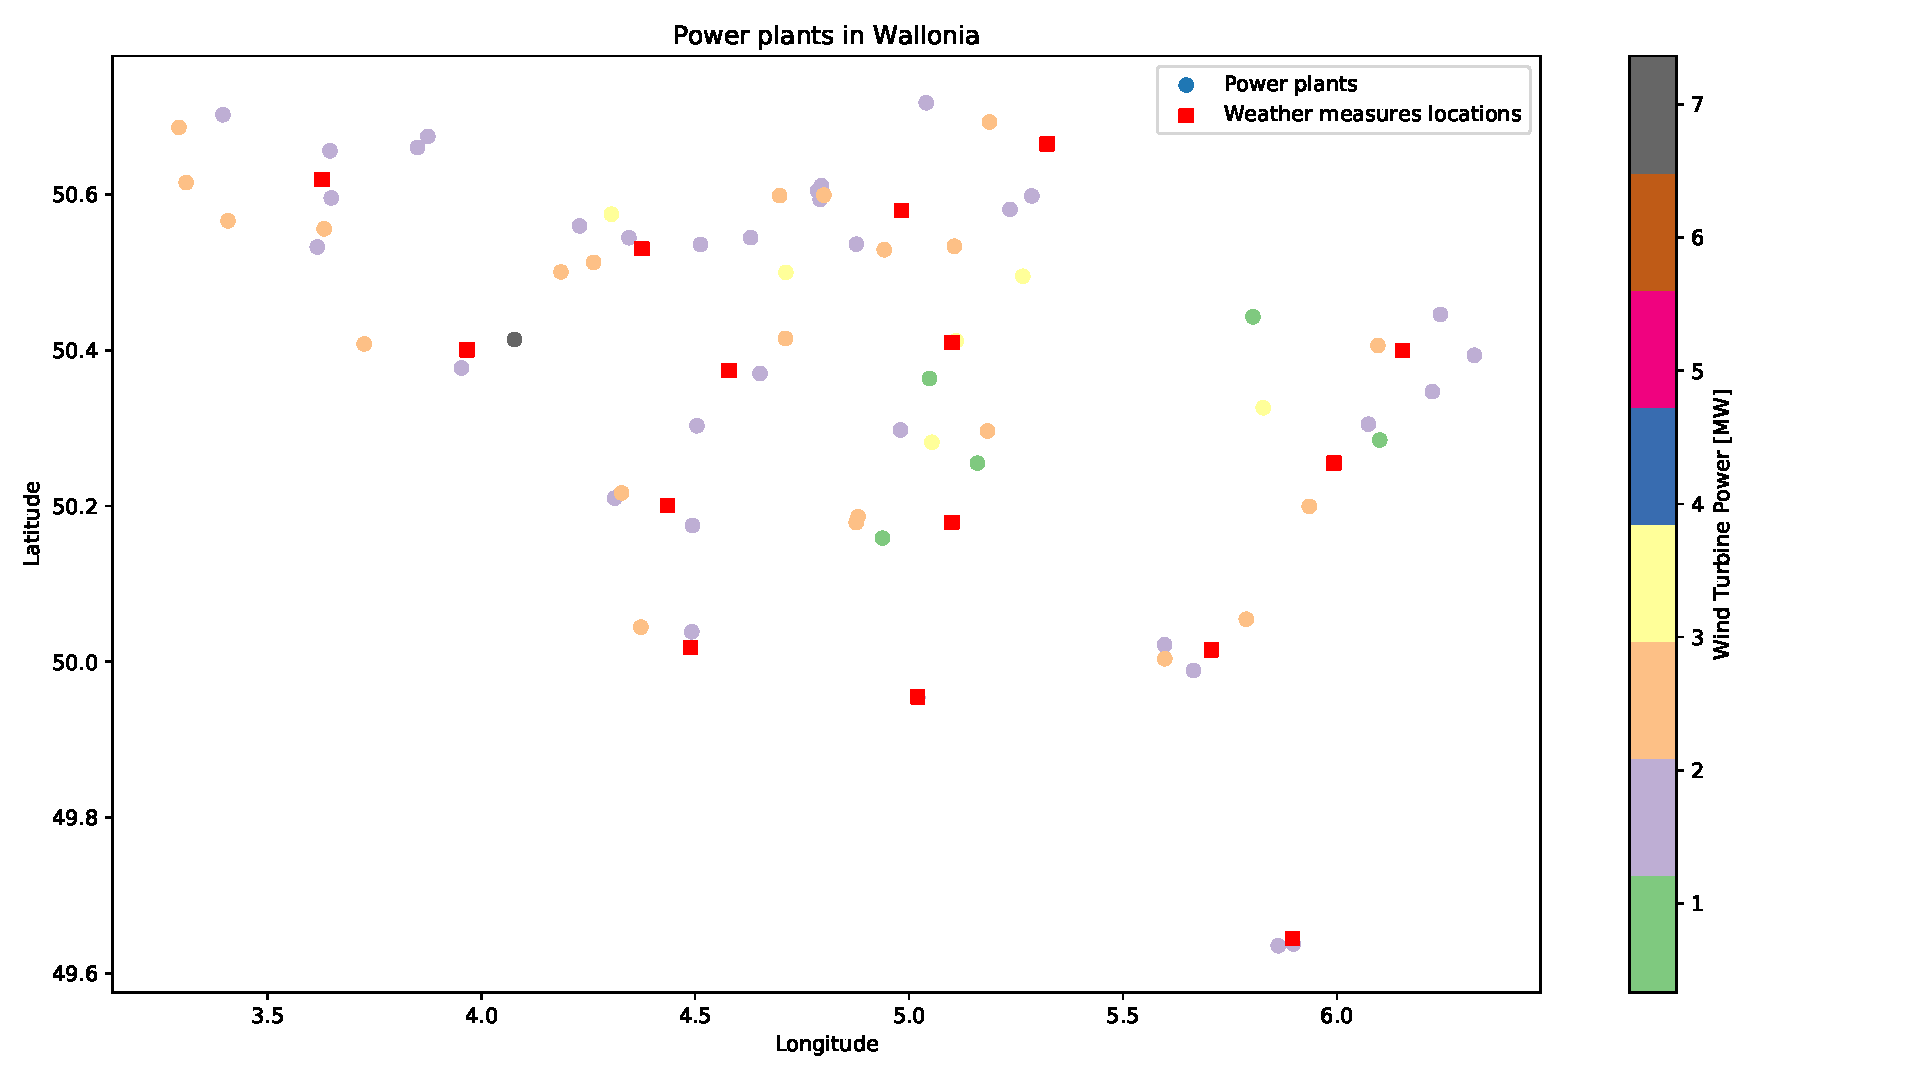
\includegraphics[width=.85\textwidth]{resources/pdf/power_plants.pdf}
        \caption{Power Plants and weather measures in Wallonia}
        \label{fig:power_plants}
    \end{figure}
    
    The last weather variable \texttt{airDensity} has been computed from the other ones, as it has been considered useful as feature of the regression problem. The thermodynamics relations used are available in \cite{airdensity}.

    \subsubsection{Metrics}
    
    Typical metric for wind power forecasting are:
    \begin{itemize}
        \item sRMSE: standardized Root Mean Squared Error.
        \item sMAE: standardized Mean Absolute Error.
    \end{itemize}
    
    State-of-the-art in both metrics is around \SI{5}{\percent} for the 12 hour ahead task, 8 to \SI{10}{\percent} for the 24 hour ahead task, as can be verified in \emph{Croonenbroack and Dahl, 2014} \cite{croonenbroeck2014windpower} and \emph{Xiaochen Wang et. al, 2011} \cite{wang2011windpower}.
    
    If the cost of an error is directly proportional to the error, it is justified to use the MAE to assess a model, that is why we choose to use sMAE as metric.
    
    Furthermore, as we designed our model such that it is able to predict confidence intervals, we have to use a proper metric to assess these predicted intervals. We have chosen to use the following metric, defined in \emph{Meinshausen, 2006} \cite{meinshausen2006quantile} :
    \begin{equation*}
        L_\alpha(y, q) = \begin{cases}\alpha \abs{y - q} & \text{ if } y > q \\ (1 - \alpha) \abs{y - q} & \text{ if } y \leq q\end{cases}
    \end{equation*}
    where $\alpha$ denotes the percentile and $q$ the predicted quantile.

    \subsubsection{Protocol}
    
    For now, two protocols have been used to choose and assess our models. Both protocols used the data between January 2019 and February 2020.  
    \begin{itemize}
        \item Protocol 1: model selection and training on the 13 first months and testing on  February 2020.
        \item Protocol 2: model selection and training on a subset randomly drawn from thirteen fourteenth of the data, testing on the rest.
    \end{itemize}

    \subsubsection{Models and results}
    
    As the data has no temporal variable such that we do not have the need to extrapolate, we focused on tree-based methods as it seemed to perform better than other methods. The two considered models are 
    \begin{itemize}
        \item Extra Trees regressor (tree bagging method)
        \item Gradient Boosting regressor (tree boosting method)
    \end{itemize}
    
    The hyperparameters of these models have been determined by cross-validation on the train set. The best obtained scores are listed in the table \ref{tab:cv_train}.
    
    \begin{table}[H]
        \centering
        \begin{tabular}{|c|c|c|}
            \hline 
            MAE & Extra Trees & Gradient Boosting \\ \hline
            Protocol 1 & 36.35 & 36.93 \\ \hline
            Protocol 2 & 25.37 & 28.18 \\ \hline
        \end{tabular}
        \noskipcaption{Train set CV scores}
        \label{tab:cv_train}
    \end{table}
    
    The results on the test set are listed in the table \ref{tab:test_scores}. Theses scores include the MAE and sMAE, together with the scores of the \SI{10}{\percent} are \SI{90}{\percent} quantiles using the loss defined earlier. 
    
    \begin{table}[H]
        \centering
        \begin{tabular}{|c|c|c|c|c|c|}
            \hline
            Protocol & Method & MAE & sMAE & MQL10 & MQL90 \\ \hline
            \multirow{2}{*}{Protocol 1} & Extra Trees & 42.38 & 6.00\% & 63.06 & 61.99 \\ \cline{2-6}
             & Gradient Boosting & 43.08 & 6.10\% & 58.91 & 43.96 \\ \hline
            \multirow{2}{*}{Protocol 2} & Extra Trees & 28.13 & 4.03\% & 46.63 & 50.32 \\ \cline{2-6}
             & Gradient Boosting & 31.11 & 4.46\% & 48.32 & 47.91 \\ \hline
        \end{tabular}
        \noskipcaption{Test set scores}
        \label{tab:test_scores}
    \end{table}
    
    These results are quite good, as is illustrated on figures \ref{fig:wind_xt} and \ref{fig:wind_gb} (protocol 1 only). 
    
    We can notice that the sMAE obtained are very good because they are based on the weather measurement instead of the day-ahead weather prediction. Once the model will be used to make forecast based on weather prediction, the error on the NWP will increase the current sMAE. If we can assume a MAE of \SI{2.4}{\meter\per{\second}} (\emph{El-Fouly et. al, 2008} \cite{el2008one}) for the wind measurement, the sMAE should be bounded by \SI{15}{\percent} in the worst case, given the power curves derivatives. First results computed on only 1 week, with day-ahead NWP instead of measurement have shown a MAE of \num{68.19} for Extra Trees and \num{70.26} for Gradient Boosting.
    
    Then, it can be noticed that the Extra Trees and Gradient Boosting compete in term of MAE, even if the Extra Trees are slightly better. 
    However, by looking at the metrics MLQ10 and MLQ90, the Gradient Boosting method seems better on the quantile regression task. Furthermore, when we look at the figures \ref{fig:wind_xt} and \ref{fig:wind_gb}, we can see that the quantiles built by the Gradient Boosting method are much tighter, which does not seem to be reflected in the quantile loss.
    
    These observations encouraged us to prefer the Gradient Boosting method in our future forecasting refinements.
    
    \begin{figure}[H]
        \centering
        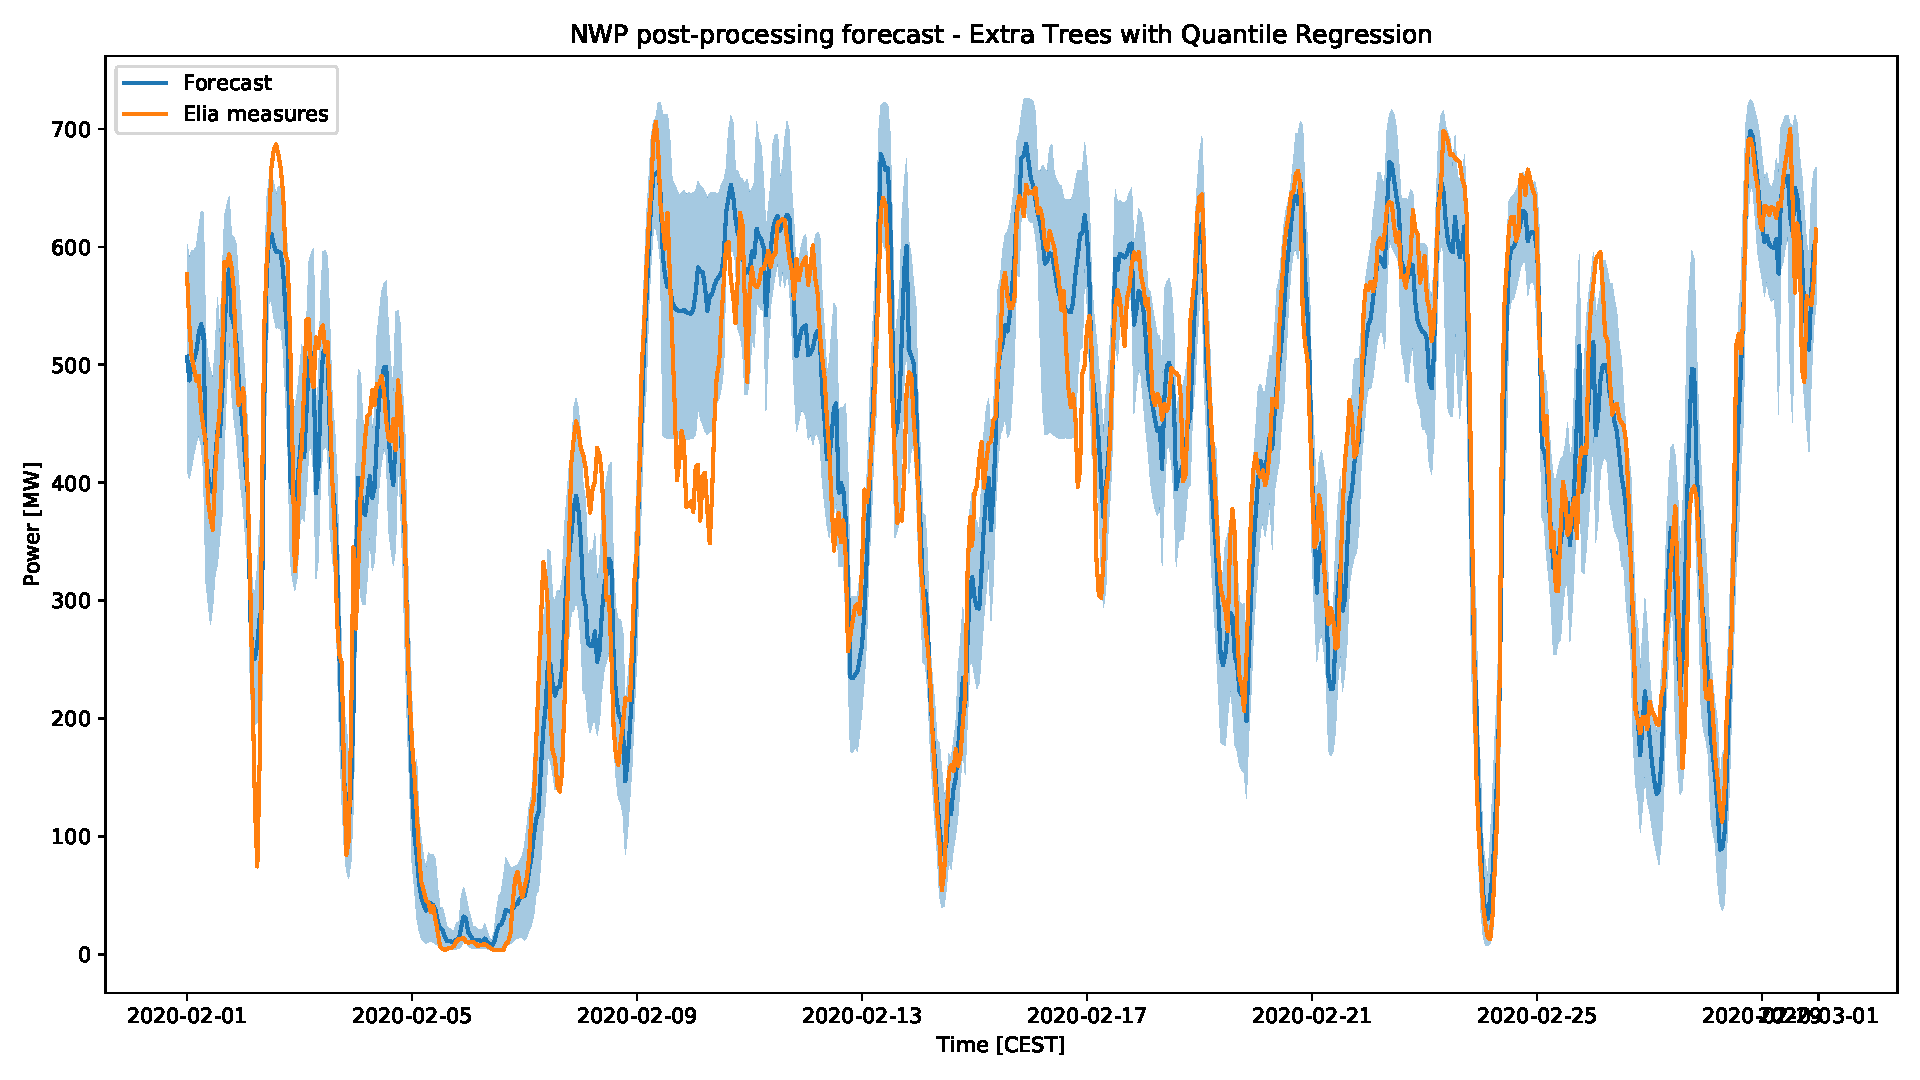
\includegraphics[width=\textwidth]{resources/pdf/wind_xt.pdf}
        \caption{Wind power forecasting - Extra Trees}
        \label{fig:wind_xt}
    \end{figure}
    
    \begin{figure}[H]
        \centering
        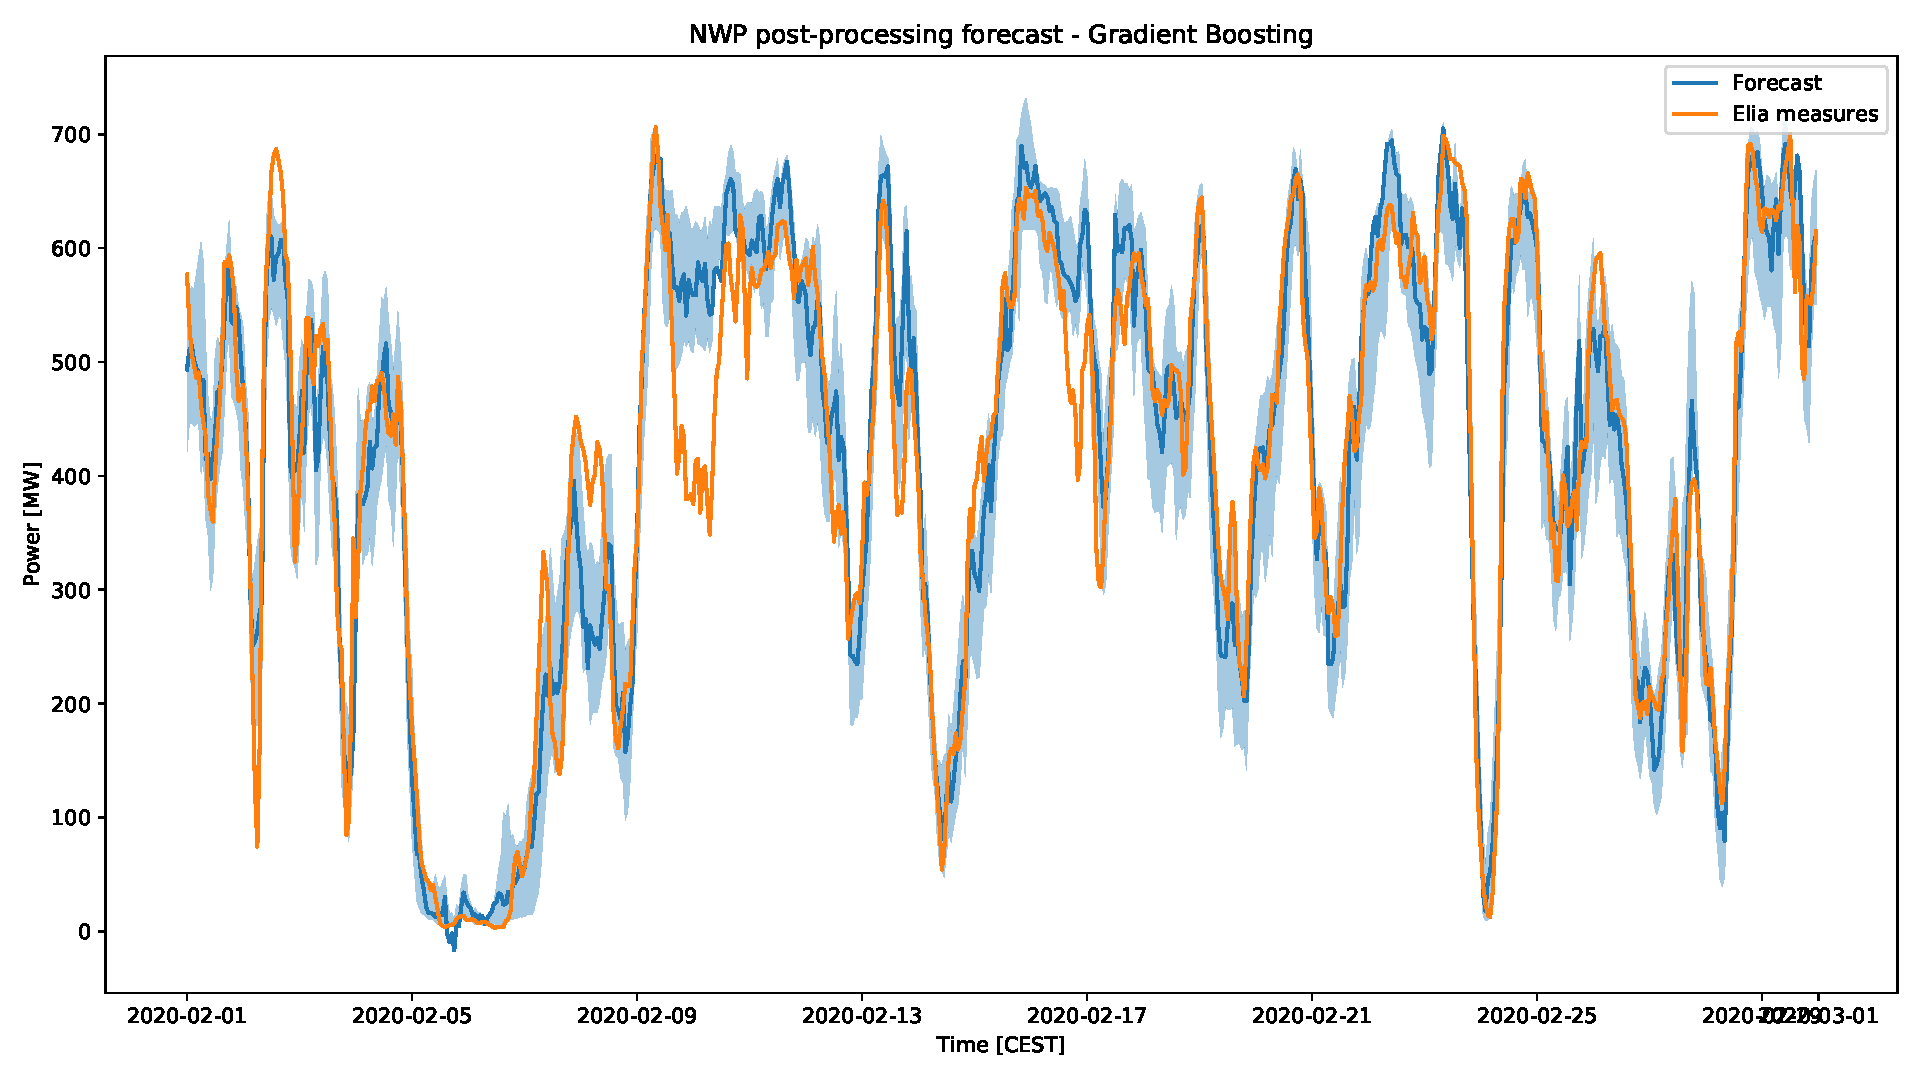
\includegraphics[width=\textwidth]{resources/pdf/wind_gb.pdf}
        \caption{Wind power forecasting - Gradient Boosting}
        \label{fig:wind_gb}
    \end{figure}
    
    \subsection{Next objectives}
    
    \begin{itemize}
        \item Including 3 new variables in the training set in order to be able to train on older data without degrading the performance :
        \begin{itemize}
            \item One-day-before power measurement (because there is a very strong correlation between the wind and the wind 24 hours before)
            \item Total wind power installed in Wallonia over time.
            \item Elia's monitored power over time (the total nominal power on which Elia takes its measurements: currently around \SI{900}{\mega\watt} out of the \SI{1036}{\mega\watt} of Wallonia)
        \end{itemize}
        \item Testing a Multi Layer Perceptron as learning method
        \item Having a look at the feature importances (some variables could be physically irrelevant) and considering feature selection
    \end{itemize}
    
    \newpage
	\printbibliography
	\appendix
	
	\section{U-Net evaluation samples}
	
	\begin{figure}[H]
	    \centering
	    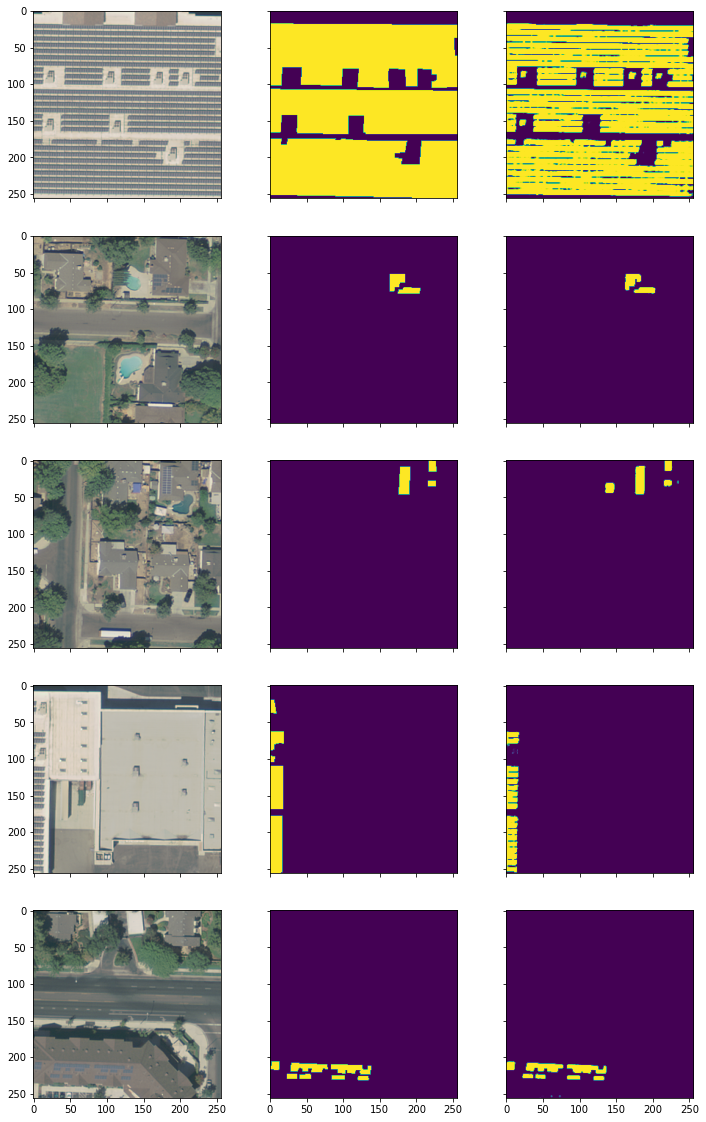
\includegraphics[height=0.92\textheight]{resources/png/representative_0.png}
	    \caption{Random sample 1}
	\end{figure}
	
	\begin{figure}[H]
	    \centering
	    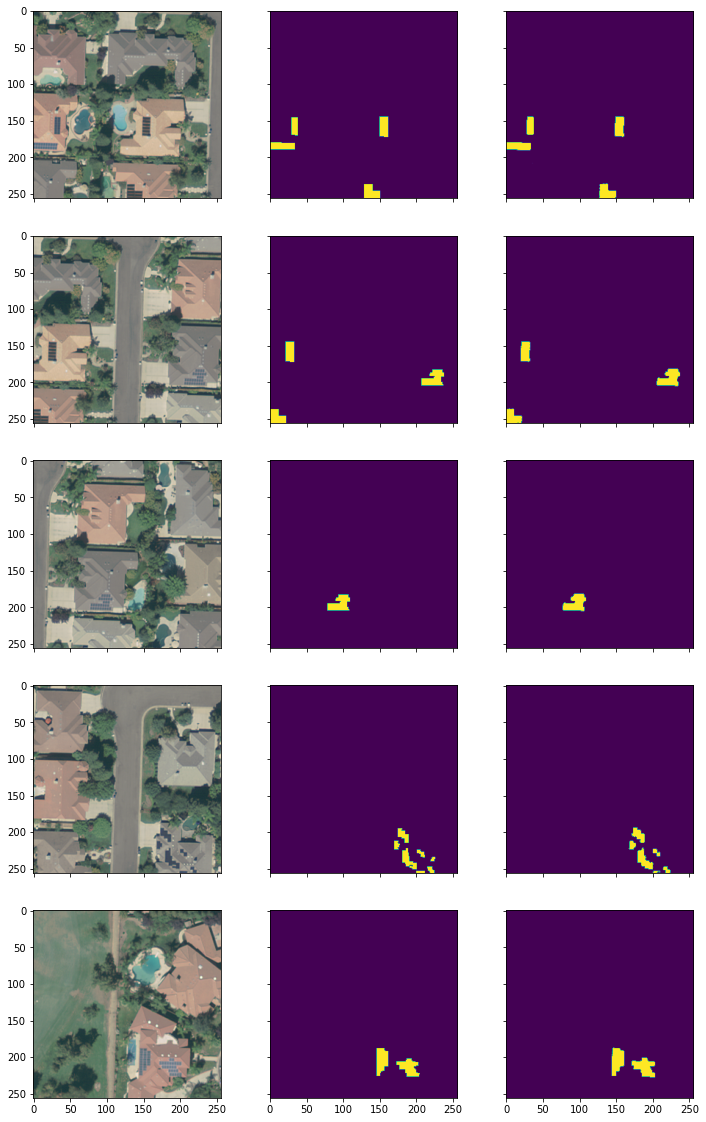
\includegraphics[height=0.92\textheight]{resources/png/representative_1.png}
	    \caption{Random sample 2}
	\end{figure}
	
	\begin{figure}[H]
	    \centering
	    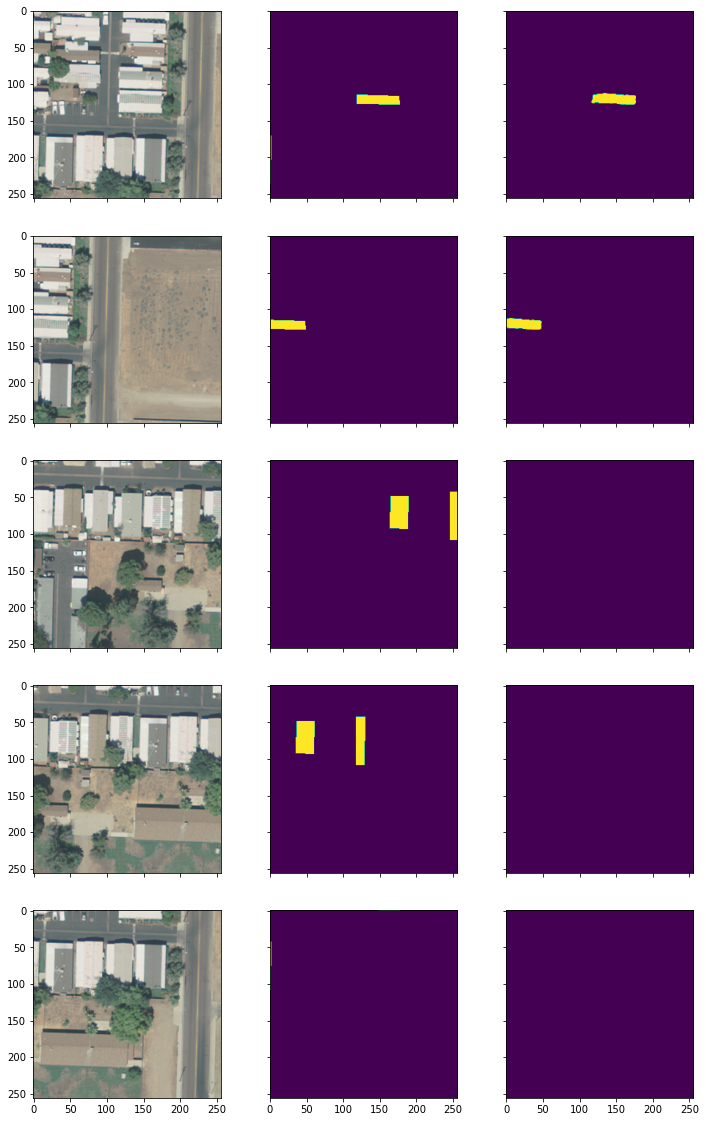
\includegraphics[height=0.92\textheight]{resources/png/bad_color.png}
	    \caption{Abnormal panel colors.}
	\end{figure}
	
	\begin{figure}[H]
	    \centering
	    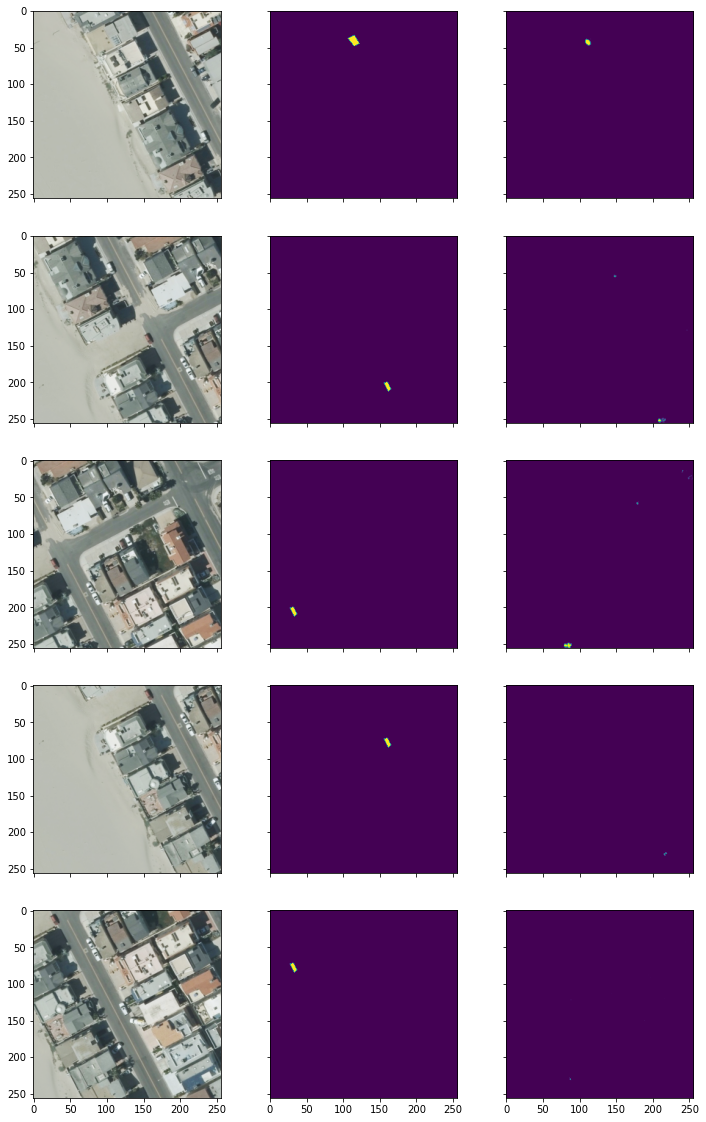
\includegraphics[height=0.92\textheight]{resources/png/bad_size.png}
	    \caption{Abnormal panel sizes.}
	\end{figure}
	
	\begin{figure}[H]
	    \centering
	    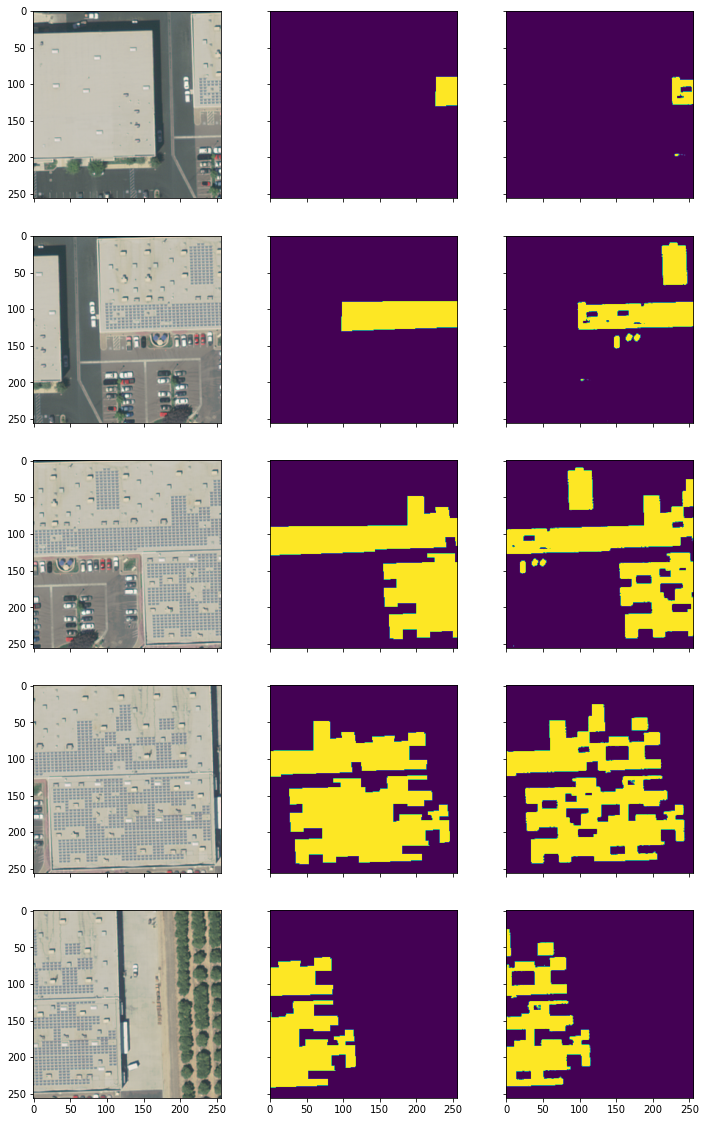
\includegraphics[height=0.92\textheight]{resources/png/beter_than_annotation.png}
	    \noskipcaption{Predictions better than annotations.}
	\end{figure}
	
	\begin{note}
	    Such annotations could be one of the causes of the relatively bad recall of our model.
	\end{note}
	
\end{document}
